\DocumentMetadata{lang=en-US, pdfversion=1.7}
\documentclass[10pt,a4paper]{extarticle}
\usepackage[margin=2.2cm]{geometry}
\usepackage{mathtools}
\usepackage{times}
\usepackage{amsmath,amssymb,amsthm}
\newtheorem{proposition}{Proposition}
\usepackage{graphicx}
\usepackage{booktabs}
\usepackage{array}
\usepackage{caption}
\usepackage[pdftitle={Blockchain-Enabled Zero Trust Identity Management for Industrial IoT with Tiered Authorization and Quorum-Governed Revocation},pdfsubject={Industrial IoT identity management, Zero Trust, blockchain},pdfkeywords={Industrial IoT; Zero Trust; Blockchain; Decentralized identifiers; Revocation governance},pdflang={en-US},pdfdisplaydoctitle=true,colorlinks=true,citecolor=blue!55!black,urlcolor=blue!55!black,linkcolor=blue!55!black]{hyperref}
\usepackage{enumitem}
\usepackage{listings}
\usepackage{xcolor}
\usepackage{setspace}
\usepackage{lineno}
\providecommand{\balance}{}
\lstset{basicstyle=\ttfamily\scriptsize,backgroundcolor=\color{gray!8},frame=single,breaklines=true,columns=fullflexible,keywordstyle=\color{blue!60!black}\bfseries,commentstyle=\color{green!40!black}}
\captionsetup{font=small,labelfont=bf}
\newcommand{\paperTitle}{Blockchain-Enabled Zero Trust Identity Management for Industrial IoT with Tiered Authorization and Quorum-Governed Revocation}
\setstretch{1.08}
\setlength{\emergencystretch}{3em}
\hfuzz=3pt
\begin{document}
\pagestyle{plain}
% ---------- Title page ----------
\begin{center}
{\Large\bfseries \paperTitle\par}
\vspace{1.2cm}
{\large Syed Irfan Raza Naqvi$^{a}$, Muhammad Umar Aftab$^{b}$, Ahmad Mohsin$^{c,*}$, Rana Asif Rehman$^{d}$, Sayed Qaiser Ali Shah$^{e}$\par}
\vspace{0.8cm}
\begin{flushleft}\small\setstretch{1.2}
$^{a}$Department of Computer Science, FAST National University of Computer and Emerging Sciences (FAST-NUCES), 852-B Faisal Town, Lahore 54770, Pakistan\\
$^{b}$Department of Computer Science, FAST-NUCES, Chiniot-Faisalabad Campus, Chiniot, Punjab, Pakistan\\
$^{c}$School of Science, Computing and Security Discipline, Edith Cowan University, 270 Joondalup Drive, Joondalup WA 6027, Australia\\
$^{d}$Faculty of Engineering and Technology, Muscat University, Muscat, Sultanate of Oman\\
$^{e}$Department of Computer Science, International Islamic University (IIU), Sector H-10, Islamabad 44000, Pakistan\\[1.2em]
$^{*}$\textbf{Corresponding author:} Dr Ahmad Mohsin, \texttt{a.mohsin@ecu.edu.au}\\[0.8em]
\textbf{Other author emails:} \texttt{l259000@lhr.nu.edu.pk}, \texttt{irfanrazanaqvi9@gmail.com}, \texttt{umar.aftab@nu.edu.pk}, \texttt{rasif@muscatuniversity.edu.om}, \texttt{qaiser.ali@iiu.edu.pk}
\end{flushleft}
\end{center}
\linenumbers
\begin{abstract}
\noindent
Industrial plants run long-lived legacy devices shared by organizations. Tokens and refreshed revocation lists fit this poorly: a revoked device keeps working until a token expires or a list refreshes, no party is trusted by all to revoke it, and one trust threshold serves every request. We present a blockchain-enabled Zero Trust architecture for industrial IoT identity management. Three contracts on a permissioned ledger hold identity and status, a tiered access policy with an anomaly gate and time-bound attestations, and quorum-voting revocation, reinstatement and recall. Gateways decide routine requests locally on replicated ledger state and high-consequence requests on-chain. We prove seven properties; the fast-path exposure bound holds only if replicas stay within an assumed lag. Counted from the submission of a revocation, both paths accepted about two requests at one request per second, against 33--147 for token and list baselines. An ablation shows that the anomaly veto does the work at the two critical tiers, cutting full-spoofing acceptance from 100\% and 53\% to 0\%; a non-linear score does the same, and an attacker that keeps its anomaly low passes every variant. With detector scores from three real datasets, the policy accepted under 1\% of seen attack types but 6.6--11.9\% of held-out types, and 29--77\% under an adaptive attacker; gates calibrated on legitimate traffic alone let 65--100\% of attacks through for an unsupervised detector. On a four-validator Besu network across four cloud regions (single runs, earlier contract version), calls were final in one 2\,s block. Posture and network signals are synthetic.
\end{abstract}
\noindent\textbf{Keywords:} Industrial IoT; Zero Trust architecture; Blockchain; Decentralized identifiers; Identity management; Smart contracts; Revocation governance
\bigskip

\section{Introduction}\label{sec:intro}

\subsection{Motivation}
An industrial plant is a poor fit for the assumptions behind most identity systems. Its devices live for fifteen or twenty years, speak protocols that predate public-key cryptography, and sit behind process-critical networks that cannot be rebooted at will. Several organizations administer them at once: the operator who runs the line, the manufacturer who ships firmware, an integrator who commissioned the cell, and sometimes an outside maintenance contractor. Guidance for operational technology (OT) security is explicit that availability and safety, not confidentiality, usually dominate the design space, and that a control that interrupts a process can be worse than the attack it prevents \cite{stouffer2023sp80082}. At the same time the attack surface has widened, because IT--OT convergence connects field assets to analytics, remote support and cloud services. Zero Trust, which drops trust based on network location and demands that every access be authenticated, authorized and re-evaluated \cite{nist800207,fernandez2024critical,phiayura2023comprehensive}, is a natural response, and early proposals adapt it to critical OT systems \cite{song2025ztot,zanasi2024flexible}.

Identity is where the difficulty concentrates. A conventional public-key infrastructure gives each device a certificate and relies on revocation lists or short certificate lifetimes to withdraw it. In a multi-party plant, however, rarely does one party hold the trust of all the others to revoke a controller. The delay between the decision to withdraw a device and the moment every gateway honours it is the window in which a compromised or recalled device keeps working. Blockchain-based identity management addresses the first problem by anchoring identifiers, keys and status on a tamper-evident ledger that several organizations operate together, following the decentralized-identifier (DID) model \cite{w3cdid2022,hosseini2023blockchain,aguru2025ssi,folino2025puf}. Recent industrial work builds authentication on this foundation \cite{zhai2025chebyshev}, and surveys of blockchain for Industrial IoT (IIoT) catalogue its promise and its open problems \cite{essaid2025iiotbc}. Studies that combine blockchain with Zero Trust have followed \cite{liu2024dissecting,nie2025zeroTrust,salim2026ztblociot,mukta2026ztdelegation,jamwal2026survey,farhan2026ztfsf,potturi2026hybrid}.

\subsection{Problem Statement and Gap}
Reading this literature with an operator's eye, three things are missing. First, most blockchain-IoT identity schemes still authenticate once and then treat the session as trusted, which is what Zero Trust is meant to remove \cite{wang2026medicaliot,james2024authz}. The Zero Trust proposals for industrial settings generally assume that one organization owns the policy decision point \cite{kumar2024industry40,zanasi2024flexible}. Second, a single trust threshold is applied to every request, although reading a temperature and rewriting a safety-controller setpoint carry very different consequences. As we show analytically and experimentally, an attacker who spoofs most of the signals can also keep a weighted score above a fixed threshold whatever its behaviour. Third, nearly all of these designs implicitly place every decision on the ledger, which cannot meet the rates and latency of plant networks. None says how to handle a manufacturer's firmware recall, a legacy device that cannot hold a key, or a lost connection to the ledger. We therefore ask:

\emph{How can a consortium-operated blockchain identity registry be combined with continuous, consequence-aware authorization so that (i) revocation, including large-scale firmware recalls, takes effect without a token or list-refresh window and without any single party being able to impose it, (ii) the strength of verification scales with the criticality of the resource, and (iii) the enforcement path stays fast, available and auditable on industrial networks?}

\subsection{Contributions}
Several elements below exist separately in earlier work (Section~\ref{sec:related}): DIDs and key-hash registries, quorum voting, Merkle-anchored logs and weighted trust scores. The new idea is to let the \emph{consequence} of a request decide where on one ledger it is decided. Routine requests are decided locally against replicated ledger state, with a proved bound on how long a revoked device can still be accepted. High-consequence requests are decided by the contract, where a finalized revocation takes effect at once. Revocation, including firmware recalls, needs a quorum, so no single registrar can impose or block it. We did not find a scheme in the literature we surveyed that combines these in one policy with a conditional exposure bound, an analysis of what the anomaly gate can and cannot stop (Proposition~\ref{prop:bound}), and measurements on a validator network. The survey is not exhaustive, so we claim a combination, not priority. The contributions are as follows.
\begin{itemize}[leftmargin=1.1em,itemsep=0pt,topsep=1pt]
  \item \textbf{Architecture.} A zone-aware design (Section~\ref{sec:arch}) with three smart contracts (identity registry, Zero Trust access policy, quorum revocation governance), a tiered policy model that ties the required trust to the criticality of the target resource, an anomaly hard gate and a strict mode for safety-relevant writes, time-bound oracle attestations, governor-only revocation with a reversible single-party quarantine, and quorum-approved batch revocation for firmware recalls. (A protocol-gateway identity proxy for legacy devices is described in Section~\ref{sec:legacy} but is not evaluated.)
  \item \textbf{Hybrid enforcement.} A two-path decision model: a fast path in which a zone gateway decides locally against replicated ledger state and anchors a Merkle root of its decision log, and an audited path in which high-consequence requests are decided by the contract itself (Section~\ref{sec:hybrid}).
  \item \textbf{Analysis.} A threat model for plant environments and seven proved properties, including a bound on how long a revoked device can still be accepted on the fast path (conditional on the replica-lag assumption A5) and a result that states when a spoofing attacker passes the anomaly gate (Sections~\ref{sec:model}--\ref{sec:security}).
  \item \textbf{Open implementation and measurement.} Solidity 0.8.24 contracts with measured gas for every operation, and a Python testbed with real Ed25519 signatures. Experiments cover revocation exposure against token, CRL and architecture-class baselines (Section~\ref{sec:prior_eval}); per-tier attack and false-denial rates, gate and weight sensitivity, quorum governance for 5--21 voters and recall capacity (Section~\ref{sec:eval}); detector scores on three real datasets, including attack types withheld from training and an adaptive attacker (Sections~\ref{sec:real_eval}--\ref{sec:wustl21_eval}); a four-validator Hyperledger Besu QBFT network, first on one host and then with one validator in each of four Google Cloud regions (Section~\ref{sec:besu_eval}); and a component ablation, exposure counted from the decision time, and gates calibrated on legitimate traffic (Section~\ref{sec:review_eval}). The network runs used an earlier version of the contracts and were single runs. We state plainly which results are compute-bound and which remain synthetic.
\end{itemize}

\section{Related Work}\label{sec:related}

\subsection{Zero Trust for Industrial and OT Systems}
Zero Trust architecture is by now well surveyed for IoT. Azad et al.\ cover continuous verification and micro-segmentation \cite{azad2024verify}, James et al.\ review authentication and authorization schemes specifically under a Zero Trust model \cite{james2024authz}, and Nahar et al.\ examine the 6G setting, where device density sharpens per-request overhead concerns \cite{nahar2024survey}. Fern\'andez and Brazhuk caution that ``Zero Trust'' is sometimes a label without a falsifiable architecture behind it \cite{fernandez2024critical}, and Phiayura and Teerakanok supply a migration framework with a maturity model \cite{phiayura2023comprehensive}. For OT in particular, Song et al.\ propose a Zero Trust architecture for critical operational technology systems \cite{song2025ztot}, and Zanasi et al.\ a flexible architecture for IIoT \cite{zanasi2024flexible}. Kumar and Sharma integrate blockchain with dynamic access control for Industry~4.0 without a DID-anchored registry \cite{kumar2024industry40}. Wei et al.\ move policy evaluation onto the client inside a zero-knowledge virtual machine, so that resource-constrained edge devices can verify a succinct proof of an XACML (eXtensible Access Control Markup Language) decision instead of relying on a costly gateway \cite{prezta2026}. These works establish the principles; they leave open who owns revocation in a multi-party plant and how a decision should be audited afterwards.

\subsection{Blockchain Identity and Authentication for IIoT}
Surveys of blockchain-based decentralized identification note limits around revocation latency and interoperability \cite{hosseini2023blockchain}, and a broad review of blockchain in IIoT discusses security and privacy opportunities alongside scalability and integration costs \cite{essaid2025iiotbc}. Aguru and Erukala propose a blockchain self-sovereign-identity framework for standardized IoT identification \cite{aguru2025ssi}, Folino et al.\ tie identity to a physically unclonable function as a hardware root of trust \cite{folino2025puf}, and Ren et al.\ combine self-sovereign identity with Zero Trust for AIoT using selective-disclosure credentials \cite{ren2025aiot}. Ali et al.\ build access management for industrial digital twins on Hyperledger Fabric with manufacturer platform-hash verification and NFT-based permission delegation, and report response times of about 300\,ms \cite{ali2025dtaccess}. On the industrial authentication side, Zhai et al.\ design a lightweight scheme for IIoT that combines blockchain with Chebyshev chaotic maps to suit constrained devices \cite{zhai2025chebyshev}. DAXiot shows that DID challenge--response for MQTT can run without a blockchain at about 21\% connection overhead over mutual Transport Layer Security (TLS), but then has no shared revocation ledger \cite{philipp2023daxiot}. For revocation itself, Mazzocca et al.\ propose EVOKE, a cryptographic-accumulator mechanism with about 1.5\,KB of per-device state that spreads revocation epidemically among devices \cite{mazzocca2024evoke}; it complements an on-chain status check rather than replacing it. Kumar et al.\ run a privacy-preserving identity system on a private Ethereum proof-of-authority (PoA) chain in which a decentralized voter group governs identity updates and revocations. They report roughly 3--4\,s for registration and under 5\,s for revocation on the live network \cite{kumar2026privacy}. This is the closest published precedent for our governance contract and the only live-chain figure we compare against.

\subsection{Blockchain--Zero Trust Combinations}
Nie et al.\ pair smart-contract policy enforcement with inner-product encryption for fine-grained access in 6G IoT \cite{nie2025zeroTrust}. Salim et al.\ propose ZT-BlocIoT with dynamic trusted gateways and reinforcement-learning-driven sharding, reporting 2{,}500 transactions per second on 700 nodes at 42\,ms latency \cite{salim2026ztblociot}. Wang et al.\ observe that even Zero Trust--inspired schemes for medical IoT typically authenticate once and then trust the session, and propose blockchain-backed continuous authentication \cite{wang2026medicaliot}; the same gap is what motivates our per-request design in industry. Rivera-Julio et al.\ screen each message after authentication, score freshness and context, and anchor Merkle roots of batched accept, challenge and revoke decisions on a modelled permissioned ledger, which is close to our decision-log anchoring but is evaluated by simulation only \cite{rivera2026yangbaxter}. Mukta et al.\ delegate Zero Trust access control through a blockchain, which is close to our policy layer but concerns delegation rather than the device identity lifecycle \cite{mukta2026ztdelegation}. For smart factories, Farhan et al.\ describe a conceptual Zero Trust framework on a consortium chain \cite{farhan2026ztfsf}, and Potturi et al.\ combine artificial intelligence (AI) risk scoring with blockchain-anchored federated identity across cloud, edge and IoT \cite{potturi2026hybrid}. Jamwal et al.\ conclude that blockchain-enabled Zero Trust is still mostly proposed at survey level rather than delivered as benchmarked open code \cite{jamwal2026survey}, and a bibliometric analysis finds blockchain with Zero Trust identity management to be one of the field's most active clusters \cite{liu2024dissecting}. Usama et al.\ add decentralized identity, zero-knowledge proofs and Byzantine-resilient federated learning against AI-driven identity attacks \cite{usama2026multilayer}. Federated learning is also studied as a way to share threat intelligence across industrial sites without exposing raw data \cite{tom2025flcti}; we do not use it, but it is a plausible source for the anomaly signal in Section~\ref{sec:signals}.

\subsection{Off-Chain Dependencies, Cost and Oracles}
Because on-chain controls rest on off-chain facts, the reliability of the data that reaches a contract matters. Shujaa et al.\ stress that device attestation, secure boot and key custody remain off-chain dependencies of any blockchain-IoT security design \cite{shujaa2025enhancing}. Hassan et al.\ survey the oracle problem, that is, how to bring trustworthy external data to a contract \cite{hassan2023oracle}. Our trust oracle is an instance of it, and Section~\ref{sec:disc} discusses its single-key weakness. Smart-contract defects are another risk, reviewed by Wei et al.\ \cite{wei2024quality}. On cost, gas has been studied for Ethereum smart contracts \cite{ta2024gascost} and for IoT access control \cite{hasan2023smartcontract}, delegated proof-of-stake (DPoS) and practical Byzantine fault-tolerant (PBFT) consensus choices have been proposed for IoT and clinical settings \cite{haque2024scalable,peepliwal2024ztab}, and gasless relaying can spare constrained devices from paying fees \cite{madhwal2025gasless}. Ren et al.\ show for vehicular networks that published trust values can themselves link pseudonyms and propose differential privacy to prevent it \cite{ren2026ditdp}, which matters for any design that exposes scores on a shared ledger.

\subsection{Positioning}
Table~\ref{tab:relatedwork} compares the most relevant systems on five properties that matter in a plant: on-chain revocation, continuous per-request authorization, consequence-aware (tiered) policy, handling of legacy and recall scenarios, and a released artifact. The assessments rest on the abstracts and the parts of the full texts we could read; ``not stated'' means we found no statement, not that the property is absent. To our knowledge none of the reviewed systems reports all five.

\begin{table*}[t]
\centering
\caption{Comparison of representative blockchain and Zero Trust systems for (I)IoT identity, as read from each paper's abstract and available text. ``n/r'' means the property is not reported there; it does not mean the system lacks it. The ``This work'' row describes what is implemented here (the legacy proxy is described but not separately evaluated)}
\label{tab:relatedwork}
\scriptsize
\resizebox{\textwidth}{!}{%
\begin{tabular}{p{3.2cm}p{3.6cm}p{1.6cm}p{1.6cm}p{1.6cm}p{2.1cm}p{1.6cm}}
\toprule
\textbf{System} & \textbf{Core mechanism} & \textbf{On-chain revocation} & \textbf{Per-request authZ} & \textbf{Tiered policy} & \textbf{Legacy / recall} & \textbf{Open artifact} \\
\midrule
Zhai et al.\ 2025 \cite{zhai2025chebyshev} & Blockchain + Chebyshev-map authentication (IIoT) & n/r & n/r & n/r & Lightweight devices & n/r \\
Song et al.\ 2025 \cite{song2025ztot} & Zero Trust architecture for critical OT & n/r & n/r & n/r & n/r & n/r \\
Zanasi et al.\ 2024 \cite{zanasi2024flexible} & Flexible Zero Trust architecture for IIoT & No & Yes & Partial & n/r & n/r \\
Kumar \& Sharma 2024 \cite{kumar2024industry40} & Blockchain + dynamic access control (Industry 4.0) & n/r & Yes & n/r & n/r & n/r \\
Farhan et al.\ 2026 \cite{farhan2026ztfsf} & ZT on consortium chain (smart factory) & Conceptual & Conceptual & n/r & n/r & n/r \\
Potturi et al.\ 2026 \cite{potturi2026hybrid} & AI risk score + chain-anchored identity & Yes & Yes & n/r & n/r & n/r \\
Salim et al.\ 2026 \cite{salim2026ztblociot} & ZT-BlocIoT (trust + DRL sharding) & Yes & Yes & n/r & n/r & n/r \\
Nie et al.\ 2025 \cite{nie2025zeroTrust} & ZT + inner-product encryption (6G) & Yes & Yes & Fine-grained attributes & n/r & n/r \\
Wang et al.\ 2026 \cite{wang2026medicaliot} & Blockchain continuous auth.\ (medical IoT) & Yes & Yes & No & n/r & n/r \\
Rivera-Julio et al.\ 2026 \cite{rivera2026yangbaxter} & Message screening + chain-anchored batched decisions (modelled ledger) & Yes (modelled) & Yes (per message) & n/r & n/r & n/r \\
Kumar et al.\ 2026 \cite{kumar2026privacy} & Private PoA identity + voter group & Yes (voter group) & n/r & No & n/r & n/r \\
\textbf{This work} & \textbf{DID registry, tiered ZT contracts, quorum governance, hybrid enforcement} & \textbf{Yes (quorum-governed, batch)} & \textbf{Yes (every call)} & \textbf{Yes (4 tiers, gate, strict)} & \textbf{Proxy identity; batch recall; outage mode} & \textbf{Yes (Solidity + Python)} \\
\bottomrule
\end{tabular}}
\end{table*}

\section{Industrial Requirements, System and Threat Model}\label{sec:model}

\subsection{Requirements Specific to Industrial Settings}\label{sec:reqs}
Translating the generic Zero Trust and blockchain-identity goals into a plant yields six requirements that drive the design; they are our reading of OT security guidance \cite{stouffer2023sp80082} and of the identity literature surveyed above, not a standard.
\begin{itemize}[leftmargin=1.1em,itemsep=0pt,topsep=1pt]
  \item \textbf{R1 Multi-party authority.} No single organization (operator, manufacturer, integrator) should be able to unilaterally revoke or reinstate a device.
  \item \textbf{R2 Consequence-aware verification.} The evidence required before a request is accepted must grow with the consequence of the target resource: reading telemetry is not rewriting a controller's program.
  \item \textbf{R3 Predictable, available enforcement.} The common-case decision must be fast and must not depend on the ledger being reachable; consensus latency is acceptable only for rare, high-consequence actions.
  \item \textbf{R4 Brownfield coexistence.} Devices that cannot hold a key or run a signature scheme must be representable without weakening the identities of those that can.
  \item \textbf{R5 Recall at fleet scale.} Withdrawing a vulnerable firmware generation must be possible for thousands of devices in a bounded number of blocks.
  \item \textbf{R6 Auditability.} Every decision, including those taken locally for speed, must be attributable and tamper-evident after the fact.
\end{itemize}
\emph{Scope.} We target the supervisory, engineering and maintenance plane: historian writes, setpoint changes, program and firmware downloads, and telemetry reads. Hard real-time cyclic I/O between a controller and its field devices, with millisecond or microsecond determinism, is outside the scope: per-message authorization there would be inappropriate, and such traffic remains protected by segmentation and by device-level mechanisms that this architecture only complements.

\subsection{System Model and Assumptions}\label{sec:sysmodel}
Devices $\mathcal{D}$ hold signing keys $(sk_i,pk_i)$ generated at commissioning, except for a \emph{legacy} subset that is represented by a protocol gateway holding a proxy identity. Zone gateways act as Policy Enforcement Points (PEPs). A trust oracle $\mathcal{O}$ with key $sk_\mathcal{O}$ attests the context signals. A registrar role is held by a provisioning service, and an optional set of $N$ voters (for example the manufacturer, the operator and an auditor) governs revocation. A consortium of $V$ validators runs a permissioned PoA chain. We assume:
\begin{itemize}[leftmargin=1.1em,itemsep=0pt,topsep=1pt]
  \item \textbf{A1 (ledger integrity).} Fewer than one third of the validators are Byzantine, the fault bound of QBFT-style consensus, so finalized state is immutable and visible to subsequent contract calls. (A simple majority of honest validators, which suffices for the voter quorum below, is \emph{not} enough for ledger safety.)
  \item \textbf{A2 (cryptography).} Ed25519 and ECDSA over secp256k1 are existentially unforgeable under chosen-message attack (EUF-CMA); SHA-256 and Keccak-256 are collision resistant.
  \item \textbf{A3 (key custody).} A device key stays secret until the adversary compromises that device. Attestation, secure boot and key custody are off-chain dependencies the ledger cannot enforce \cite{shujaa2025enhancing}.
  \item \textbf{A4 (role keys).} The policy-administrator and oracle keys are uncompromised, and at most $q-1$ voter keys are compromised.
  \item \textbf{A5 (replica freshness).} A zone replica applies each finalized registry event within $\Delta$ seconds of finality. $\Delta$ is an operational parameter (for example the block interval plus a polling or subscription delay), not a protocol guarantee.
\end{itemize}

\subsection{Adversary Model and Security Goals}\label{sec:adversary}
The adversary controls the network between devices and PEPs (observe, replay, drop, inject), may compromise a bounded set of devices and obtain their keys, may enrol devices of its own, and controls the context signals reported by a device it has compromised. It cannot break A1--A5. In addition, we consider an \emph{insider}: a single organization that holds the registrar role and tries to revoke or reinstate devices for its own advantage. Table~\ref{tab:threats} maps threats to mitigations and evidence.

\begin{table}[t]
\centering
\caption{Threat model: adversary actions, mitigations and evidence}
\label{tab:threats}
\scriptsize
\begin{tabular}{@{}p{1.9cm}p{3.3cm}p{1.8cm}@{}}
\toprule
\textbf{Threat} & \textbf{Mitigation} & \textbf{Evidence} \\
\midrule
T1 Replay & Nonce set (audited) or monotonic counter (fast path) & Prop.~\ref{prop:replay}; Sec.~\ref{sec:attacks} \\
T2 Impersonation / forgery & Signature checked against on-chain key & Sec.~\ref{sec:attacks} \\
T3 Use after revocation & Status first on every call; terminal REVOKED & Props.~\ref{prop:revoke}, \ref{prop:stale}; Sec.~\ref{sec:baselines} \\
T4 Re-enrolment of a revoked key & Key-hash blacklist & Prop.~\ref{prop:key} \\
T5 Self-declared trust or tampered anomaly value & Oracle signature over $(\mathrm{did},\mathrm{res},T,A,\mathrm{nonce})$ & Prop.~\ref{prop:oracle} \\
T6 Signal spoofing / mimicry & Bounded signal weights, anomaly gate, strict tiers & Prop.~\ref{prop:bound}; Secs.~\ref{sec:tiers_eval}, \ref{sec:gate_eval} \\
T7 Insider revokes or reinstates at will & Quorum governance & Prop.~\ref{prop:gov}; Sec.~\ref{sec:governance_eval} \\
T8 Legacy device impersonated behind a gateway & Proxy identity limited to low tiers & Sec.~\ref{sec:legacy} \\
T9 Ledger or replica outage & Tier-dependent degraded mode & Sec.~\ref{sec:outage} \\
T10 Validator collusion, oracle compromise & Out of scope (A1, A4) & Sec.~\ref{sec:disc} \\
\bottomrule
\end{tabular}
\end{table}

The goals are: \textbf{G1} no request is accepted from a revoked, suspended or unknown identity, immediately on the audited path and within $\Delta$ on the fast path; \textbf{G2} each request is accepted at most once; \textbf{G3} a device cannot raise its own trust or lower its own anomaly value; \textbf{G4} a compromised key cannot be reused under a new identity; \textbf{G5} the effect of any single context signal, and the conditions under which a spoofing attacker is accepted, are known exactly; \textbf{G6} fewer than $q$ voters cannot revoke a device, and fewer than $N-q+1$ cannot block a revocation that $q$ voters approve; and \textbf{G7} every decision, including fast-path ones, is covered by an anchored commitment.

\section{Proposed Architecture}\label{sec:arch}

\subsection{Overview}
Figure~\ref{fig:arch} shows the design. Devices and a protocol gateway sit in the field zone; the zone PEP enforces decisions; the trust engine (policy decision point, PDP), trust oracle and a local replica of the chain state sit in the site operations zone; and the three contracts are operated by the consortium. The PEP/PDP split follows the classical Zero Trust reference model \cite{nist800207,fernandez2024critical}, but the policy store and the identity registry are held by the consortium rather than by one site, so that no gateway can edit another stakeholder's view of a device.

\begin{figure*}[t]
\centering
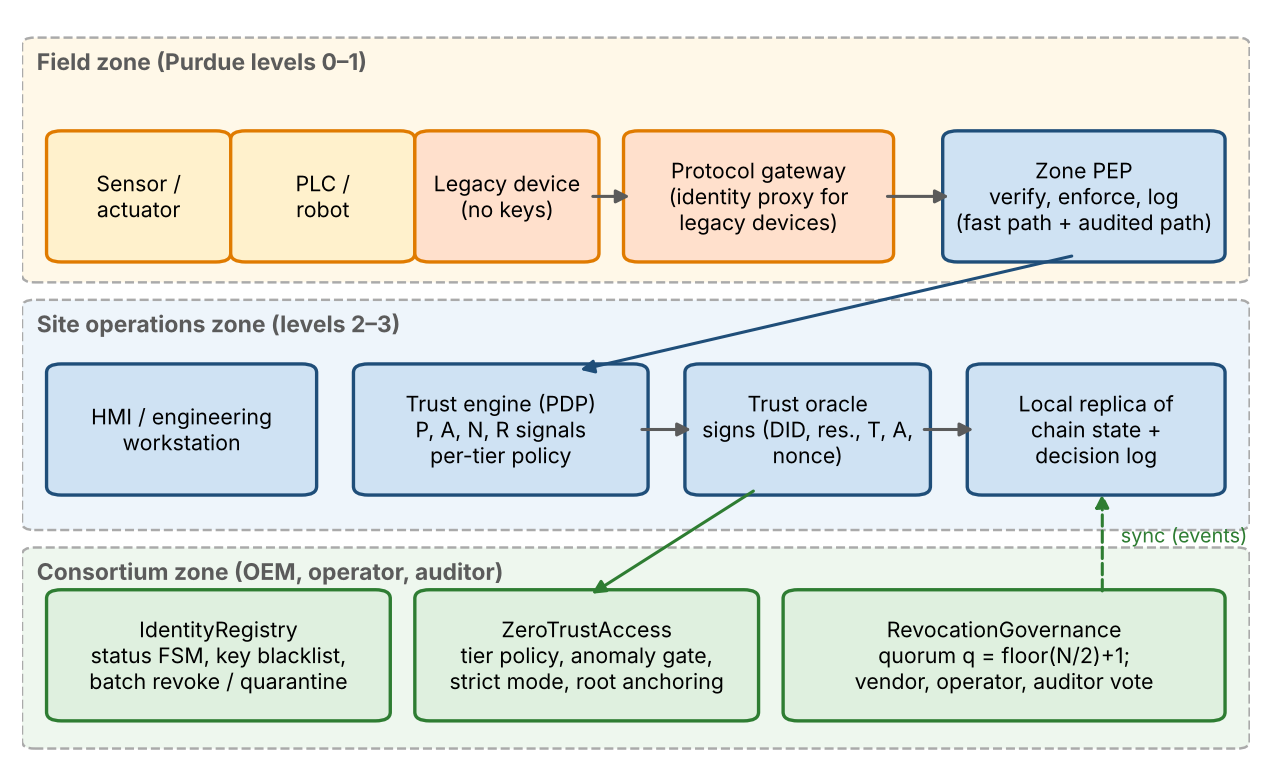
\includegraphics[width=0.72\textwidth]{../figures/fig7_iiot_arch.png}
\caption{Architecture of the blockchain-enabled Zero Trust system for Industrial IoT identity management, organized by plant zone. Text description: three stacked zones. The field zone holds sensors, PLCs, legacy devices, a protocol gateway and the zone PEP (fast and audited paths); the site operations zone holds the trust engine, trust oracle and a local chain replica for the fast path; the consortium zone holds the three contracts, whose events synchronize the replica. Arrows: (1) signed request, (2) context to the trust engine, (3) score and anomaly signal to the oracle, (4) signed attestation on the audited path (T2--T3), (5) chain state for the fast path (T0--T1), (6) contract events to the replica.}
\label{fig:arch}
\end{figure*}

\subsection{Identity Lifecycle and the Registry}\label{sec:identity}
A device derives a DID from its public key in the style of the W3C data model \cite{w3cdid2022}, $\mathrm{did}=\texttt{did:iot:}\,\mathrm{H}(pk)[0{:}32]$, with SHA-256 in the testbed and Keccak-256 in the Solidity track. Commissioning submits $pk$ (or its hash), a device class, and a hash of the declared attributes (firmware version, vendor, location), signed by $sk$ so that the record proves key possession without exposing the attributes. The registry is a state machine:
\[
\text{UNKNOWN} \xrightarrow{\text{register}} \text{ACTIVE}
\]
\[
\text{ACTIVE} \xrightarrow{\text{suspend}} \text{SUSPENDED} \xrightarrow{\text{reinstate}} \text{ACTIVE}
\]
\[
\text{ACTIVE or SUSPENDED} \xrightarrow{\text{revoke}} \text{REVOKED (terminal)}
\]
REVOKED is terminal, and revocation also blacklists the key hash, so the same key cannot be enrolled under a new DID. Suspension is the reversible quarantine used while an advisory is assessed. Every transition emits an indexed event, which zone replicas and security monitoring consume. Authority is split by consequence: the registrar role may \texttt{register} and \texttt{suspend} (a reversible quarantine), whereas \texttt{revoke}, \texttt{reinstate} and batch revocation are restricted to a \emph{governor} role. At deployment the administrator calls \texttt{lockGovernance(governance)}, which makes the governance contract the only governor and removes the administrator's own; from then on a single party can quarantine a device but cannot permanently revoke or reinstate one.

\subsection{Legacy Devices Behind a Protocol Gateway}\label{sec:legacy}
Brownfield equipment often cannot sign requests. We represent each such device by a DID derived from the \emph{gateway's} key and the device's local address, registered with the class \texttt{legacy}. The gateway signs on its behalf and supplies weaker posture evidence (the testbed draws legacy posture from a lower range than native devices). Two rules keep this from lowering the security of the whole plant: the class check admits \texttt{legacy} identities only to low-consequence resources (tiers T0--T1 in our policy), and revoking the gateway key revokes every proxied identity at once. The trade-off is explicit: a compromised gateway can speak for every legacy device behind it, which is why this class never reaches the strict tiers.

\subsection{Tiered Zero Trust Policy}\label{sec:tiers}
Each resource has a policy $\pi=(\theta,m,g,s,\mathcal{C},\tau_{\max})$: a minimum trust $\theta$, a step-up margin $m$, an anomaly hard gate $g$, a strict flag $s$, a set of permitted device classes $\mathcal{C}$ and a maximum idle time $\tau_{\max}$. Table~\ref{tab:tiers} lists the four tiers used in our evaluation. The parameters are illustrative and tuned by hand to our synthetic signal ranges; a real plant would set them from its own telemetry and risk assessment.

\begin{table}[t]
\centering
\caption{Criticality tiers used in the evaluation (HMI, human--machine interface; PLC, programmable logic controller)}
\label{tab:tiers}
\scriptsize
\begin{tabular}{@{}llcccl@{}}
\toprule
\textbf{Tier} & \textbf{Example resource} & $\theta$ & $m$ & $g$ & \textbf{Classes} \\
\midrule
T0 & telemetry.read & 0.50 & 0.10 & 1.00 & all, incl.\ legacy \\
T1 & historian.write & 0.55 & 0.10 & 0.60 & all but HMI \\
T2 & plc.setpoint.write$^{\dagger}$ & 0.70 & 0.05 & 0.30 & HMI, PLC, robot \\
T3 & plc.firmware.update$^{\dagger}$ & 0.78 & 0.04 & 0.20 & PLC, robot \\
\bottomrule
\multicolumn{6}{l}{$^{\dagger}$ strict: borderline scores are denied rather than stepped up.}
\end{tabular}
\end{table}

The trust score combines four signals in $[0,1]$: device posture $P$ (attested firmware and configuration state), behavioural anomaly $A$, network context $N$ and historical reliability $R$ (mean of the last ten scores, 0.6 for a new device),
\begin{equation}
T=w_pP+w_b(1-A)+w_nN+w_rR,\label{eq:score}
\end{equation}
with default weights $(w_p,w_b,w_n,w_r)=(0.30,0.30,0.20,0.20)$,
\label{sec:signals}The signals come from the PEP and from monitoring that the plant already operates. In practice $A$ could be produced by process-aware anomaly detection, possibly trained across sites without sharing raw data \cite{tom2025flcti}. We treat their production as an input and evaluate only how the policy handles them. The oracle signs $(\mathrm{did},\mathrm{res},T,A,t_{\mathrm{valid}},\mathrm{nonce})$, where $t_{\mathrm{valid}}$ is an expiry time; including $A$ in the signed message lets a contract enforce the gate without trusting the device's own report. The expiry bounds how long a captured attestation of a good score stays usable.

\begin{center}
\begin{minipage}{\linewidth}
\small
\textbf{Algorithm 1} \texttt{evaluateAccess(did, res, class, T, A, $t_{\mathrm{valid}}$, nonce, sig)}
\begin{enumerate}[leftmargin=1.4em,itemsep=0pt,topsep=2pt]
  \item \textbf{if} status(did) $\ne$ ACTIVE \textbf{or} no policy for res \textbf{then return} DENY
  \item \textbf{if} (did, nonce) already used \textbf{then return} DENY; mark it used
  \item \textbf{if} class $\notin\mathcal{C}$ \textbf{then return} DENY
  \item \textbf{if} the block time exceeds $t_{\mathrm{valid}}$ \textbf{then return} DENY \hfill\textit{(attestation expired)}
  \item \textbf{if} oracle signature over (did, res, $T$, $A$, $t_{\mathrm{valid}}$, nonce) is invalid \textbf{then return} DENY
  \item \textbf{if} $A>g$ \textbf{then return} DENY \hfill\textit{(anomaly gate)}
  \item \textbf{if} $T<\theta$ \textbf{then return} DENY
  \item \textbf{if} $T<\theta+m$ \textbf{then return} (\textbf{if} strict \textbf{then} DENY \textbf{else} STEP\_UP)
  \item \textbf{return} ALLOW
\end{enumerate}
\end{minipage}
\end{center}

The gate and the strict flag address a weakness of weighted scores that Proposition~\ref{prop:bound} makes precise. Because the score is linear, an attacker who spoofs posture, network and reliability can hold $T$ high however abnormal its behaviour is. For consequential resources the anomaly signal must therefore be able to veto independently of the sum. For a step-up, we leave the second-factor mechanism to the plant (for example a local operator confirmation); STEP\_UP is never returned for strict resources.

\subsection{Hybrid Enforcement: Fast Path and Audited Path}\label{sec:hybrid}
Running Algorithm~1 on the chain for every request would cap throughput at what a block can carry and would couple plant operations to consensus latency. We therefore split enforcement by tier.
\begin{itemize}[leftmargin=1.1em,itemsep=0pt,topsep=1pt]
  \item \textbf{Fast path (T0, T1).} The zone PEP decides locally against its replica: status and key from the registry events, a per-device monotonic counter in place of the nonce set, the device's request signature, the oracle's attestation and the tier policy. Each decision appends a leaf to a log; every $B$ decisions the PEP computes a Merkle root and anchors it with \texttt{anchorDecisions(root, count)}, which only authorized PEP addresses may call. An auditor can later check any single logged decision against the anchored root.
  \item \textbf{Audited path (T2, T3).} The request is decided by \texttt{evaluateAccess} on the chain, so the decision, its inputs and its outcome are themselves on the ledger. These resources are written rarely and under operator control, which is what makes the cost acceptable; if a plant's setpoint writes are frequent, this assumption fails and the tiers must be re-cut.
\end{itemize}
The price of the fast path is the replica lag $\Delta$ of assumption A5: a device revoked just before a request may still be accepted for tier T0--T1 resources until the replica catches up (Proposition~\ref{prop:stale}). The audited path has no window after finality, but it is not instantaneous either, because the revocation must first be included in a block. Measured from the moment a revocation is \emph{submitted}, the exposure is of the same order on both paths (Section~\ref{sec:exposure_eval}).

\subsection{Firmware Recall and Quarantine}\label{sec:recall}
When a vulnerability is disclosed in a firmware generation, the manufacturer needs to withdraw every affected device quickly. A recall is a governed action. A voter calls \texttt{proposeBatch(batchHash, reason)} with the hash of the device list; when $q$ voters approve, anyone may call \texttt{executeBatch(proposalId, dids)}, which checks the list against the approved hash, runs once, and calls \texttt{revokeBatch} on the registry (which skips unknown or already-revoked entries rather than reverting, blacklists each key and emits one event per device). \texttt{suspendBatch} lets a single registrar quarantine a fleet reversibly while the vote is pending. The batch is limited by the block gas limit, and Section~\ref{sec:recall_eval} measures its per-device gas and the number of blocks needed for fleets of $10^3$--$5\times10^4$ devices.

\subsection{Decentralized Revocation Governance}\label{sec:governance}
A single registrar can deny service to legitimate devices, or reinstate a dangerous one. \texttt{RevocationGovernance} therefore mediates every permanent or restoring action through threshold voting among $N$ independent voters, in the spirit of the voter group of \cite{kumar2026privacy}. A voter calls \texttt{propose(did, reason)}, \texttt{proposeReinstate(did)} or \texttt{proposeBatch(batchHash, reason)}; each voter casts one \texttt{castVote(id, approve)}. A proposal executes as soon as approvals reach $q=\lfloor N/2\rfloor+1$, and is finalized as rejected once denials exceed $N-q$. After \texttt{lockGovernance} the governance contract is the only governor, so there is no direct path: a time-critical response by one party is limited to \texttt{suspend}. Votes are non-transferable, one per voter, and DENY votes never count toward approval. We have not implemented voter-set changes, proposal expiry or key rotation for voters or the oracle; liveness requires that at least $q$ voters take part, so $q$ unavailable or unwilling voters block a revocation (the single-party \texttt{suspend} remains available meanwhile).

\subsection{Degraded Operation During an Outage}\label{sec:outage}
If a PEP loses its replica feed, it must pick between availability and safety. Our policy is tier-dependent: T0--T1 requests continue against the last known state (accepting that a device revoked during the outage is not yet known), while audited-path requests (T2--T3) are \emph{denied}, because their decision needs the chain. This is fail-closed for consequential writes and fail-operational for reads; whether an operator accepts that trade is a plant decision, and Section~\ref{sec:outage_eval} quantifies it for a simple scenario.

\section{Security Analysis}\label{sec:security}
The contracts are deterministic state machines, so the proofs are short; they establish that the logic meets goals G1--G7 under A1--A5, not that a deployment is secure.

\subsection{Security Properties}\label{sec:props}
\begin{proposition}[Immediate revocation on the audited path, G1]\label{prop:revoke}
If \texttt{revokeDevice(did)} (or \texttt{revokeBatch} containing \texttt{did}) is in a finalized block, every later call to \texttt{evaluateAccess} for \texttt{did} returns DENY.
\end{proposition}
\emph{Proof.} By A1 the call sees finalized state with $\mathrm{status}(\mathrm{did})=$ REVOKED. No function leaves REVOKED, and step~1 of Algorithm~1 runs before every other check and denies all non-ACTIVE statuses. \hfill$\square$

\begin{proposition}[Bounded exposure on the fast path, G1]\label{prop:stale}
Let a revocation finalize at time $t_f$ and let a PEP satisfy A5 (this is an assumption about the deployment, not something the contracts guarantee: if the replica lags more than $\Delta$, the bound fails). A fast-path request evaluated at time $\tau\ge t_f+\Delta$ is denied. If the device submits at most $\rho$ accepted requests per second, at most $\rho\Delta$ requests are accepted after $t_f$.
\end{proposition}
\emph{Proof.} By A5 the replica shows status REVOKED from $t_f+\Delta$ on, and the fast path denies non-ACTIVE devices before any other check. Requests accepted after $t_f$ therefore fall in $[t_f,t_f+\Delta)$, which holds at most $\rho\Delta$ of them. \hfill$\square$

\begin{proposition}[Replay resistance, G2]\label{prop:replay}
For a single PEP and any $(\mathrm{did},c)$ with $c$ a nonce (audited) or counter value (fast path), at most one evaluation returns ALLOW or STEP\_UP.
\end{proposition}
\emph{Proof.} Audited path: the test-and-set of the used-nonce flag is one transaction and transactions execute serially, so a second evaluation sees the flag and denies at step~2. Fast path: the PEP accepts only counters greater than the stored maximum and then stores the new value, so a repeated or older counter is denied. In a multi-PEP zone, the PEP identity must be bound into the signed message so that a request captured at one PEP is useless at another; our testbed exercises a single PEP. \hfill$\square$

\begin{proposition}[Attestation unforgeability, G3]\label{prop:oracle}
A PPT adversary without $sk_\mathcal{O}$ obtains ALLOW or STEP\_UP for a pair $(T,A)$ not attested by $\mathcal{O}$ for that request only with negligible probability.
\end{proposition}
\emph{Proof.} The score checks are reached only after the attestation has not expired and its signature over $(\mathrm{did},\mathrm{res},T,A,t_{\mathrm{valid}},\mathrm{nonce})$ verifies under $pk_\mathcal{O}$. Producing a different $(T,A)$, or a later $t_{\mathrm{valid}}$, with a valid signature is an EUF-CMA forgery (A2). The nonce is inside the message, so an attestation cannot be moved to another request, and the expiry means a good score attested long ago cannot be presented after the device has degraded. Changing only $A$ or only $t_{\mathrm{valid}}$ changes the signed message, which the contract tests demonstrate. \hfill$\square$

\begin{proposition}[Key-reuse prevention, G4]\label{prop:key}
After a finalized revocation, \texttt{registerDevice} with the same key hash reverts.
\end{proposition}
\emph{Proof.} Revocation sets $\mathrm{revokedKey}[\mathrm{H}(pk)]$, and registration reverts on that flag. Since the DID is a function of $\mathrm{H}(pk)$, a new identity needs a new key, which the adversary lacks unless it compromised another device. \hfill$\square$

\begin{proposition}[Governance safety and liveness, G6]\label{prop:gov}
With $N$ voters, quorum $q$, and governance locked: (a) a revocation, reinstatement or batch recall executes only if at least $q$ distinct voters approved it; (b) a set of at most $N-q$ voters cannot stop a proposal that the other $q$ approve; (c) a coalition of at most $q-1$ voters cannot execute any of these actions; (d) no single party, including the administrator, can revoke or reinstate a device, and the most a registrar can do alone is suspend.
\end{proposition}
\emph{Proof.} (a) \texttt{hasVoted} blocks repeats and \texttt{isVoter} blocks outsiders; the approval counter reaches $q$ only with $q$ distinct approvals, and only then is \texttt{revokeDevice} called. (b) Denials end a proposal only when they exceed $N-q$, which at most $N-q$ dissenters cannot, so the $q$ approvers can always complete. (c) Fewer than $q$ approvals never trigger execution. (d) After \texttt{lockGovernance} the registry's governor set is exactly the governance contract, and \texttt{revokeDevice}, \texttt{revokeBatch} and \texttt{reinstateDevice} are the only functions that reach REVOKED or leave SUSPENDED; the contract tests check that the former administrator is rejected. Liveness is conditional: it needs at least $q$ voters to participate. \hfill$\square$

\begin{proposition}[Spoofing, the gate and strictness, G5]\label{prop:bound}
(a) If scores $T,T'$ differ only in signal $s_j$ with weight $w_j$, then $|T-T'|\le w_j$. (b) On a resource with gate $g$, every ALLOW satisfies $A\le g$. (c) On a strict resource, every ALLOW satisfies $T\ge\theta+m$. (d) For an attacker with $P=N=R=1$, $T=1-w_bA$, and it is accepted on a strict resource if and only if $A\le\min\{g,(1-\theta-m)/w_b\}$.
\end{proposition}
\emph{Proof.} (a) $T-T'=w_j(s_j-s_j')$ and $|s_j-s_j'|\le1$. (b) and (c) are steps 5 and 7 of Algorithm~1. (d) Substituting gives $T=0.3+0.3(1-A)+0.2+0.2=1-0.3A$, and ALLOW needs $A\le g$ and $T\ge\theta+m$. \hfill$\square$

\emph{Corollary (what a fixed threshold cannot do).} With the default weights a fully spoofing attacker has $T\ge0.70$ even at $A=1$. Hence on a non-strict resource with $\theta=0.55$ and no gate, \emph{no} anomaly value gets such an attacker denied. For the tiers of Table~\ref{tab:tiers} the bound $(1-\theta-m)/w_b$ is $0.83$ (T2) and $0.60$ (T3), above the gates $0.30$ and $0.20$. The \emph{gate}, not the score, is what stops the attacker, and the residual risk is the set of attackers who keep $A\le g$. The experiments of Section~\ref{sec:gate_eval} measure how that residual behaves.

\subsection{Trust Anchors: Oracle, Voters and Collusion}\label{sec:anchors}
The guarantees rest on two trusted parties that the design does not remove. \emph{The trust oracle} signs the context signals. If its key is stolen, an attacker can attest any posture and network context, which defeats the gate (Proposition~\ref{prop:bound}(d)) but not revocation or replay protection, because the status and nonce checks do not use the oracle. Oracle compromise therefore degrades continuous authorization to signature plus status. A threshold-signed oracle ($t$ of $n$ attesters run by different organizations) with periodic key rotation recorded as a role change is the remedy; we recommend it but have not implemented it. \emph{The voters} are the named consortium members (for example manufacturer, operator and auditor). In our contracts the voter set is fixed at deployment; admitting or removing a voter should itself need the same quorum, which we do not implement. Governance bounds what colluding voters can do: fewer than $q$ cannot revoke any device (Proposition~\ref{prop:gov}), but $q$ or more can revoke any device, which is a denial of service against the plant. Sybil voters are excluded by admission, not by cryptography: voters are identified organizations that join by agreement, so that defence is legal and organizational and the chain cannot enforce it. Choosing $N$ and $q$ is therefore a governance decision, since a larger $N$ raises the collusion threshold and the gas cost (313k--800k gas for $N=5$--$21$).

\subsection{Alignment with the NIST Zero Trust Tenets}\label{sec:tenets}
Table~\ref{tab:tenets} maps the seven tenets of NIST SP~800-207 \cite{nist800207} onto the design and states where it falls short.

\begin{table}[t]
\centering
\caption{Design against the seven NIST SP~800-207 tenets}
\label{tab:tenets}
\scriptsize
\begin{tabular}{@{}p{2.2cm}p{1.1cm}p{3.6cm}@{}}
\toprule
\textbf{Tenet} & \textbf{Status} & \textbf{How, and where it stops} \\
\midrule
1 All data sources and services are resources & Partial & Device-to-resource requests are covered by criticality tier; users and applications are out of scope. \\
2 All communication is secured regardless of location & Not covered & Requests are signed and replay-protected; channel confidentiality (TLS, OPC UA security) is assumed off-chain. \\
3 Access is granted per session & Met, stricter & Decided per request, not per session. \\
4 Access follows dynamic policy (identity, device state, behaviour) & Met & Tiered score of behaviour, posture, network and reliability; posture and network inputs are synthetic in our experiments. \\
5 Integrity and posture of all assets are monitored & Partial & Posture is an oracle-attested input; attestation and monitoring are off-chain dependencies (A3). \\
6 Authentication and authorization are dynamic and enforced before access & Met & Signature, status and policy are checked before each decision; the fast path has the bounded exposure of Proposition~\ref{prop:stale}. \\
7 Information on assets, traffic and access is collected to improve posture & Partial & Decisions are logged and anchored; telemetry collection and policy learning are not evaluated. \\
\bottomrule
\end{tabular}
\end{table}

\subsection{Residual Risks}\label{sec:residual}
The properties say nothing about (i) compromised validators or oracle keys (A1, A4); (ii) a stolen key used by an attacker who behaves like the owner until revoked, which no continuous scheme separates from the owner except by behaviour; (iii) side-channel extraction of keys; or (iv) smart-contract defects, for which the quality-assurance literature recommends testing, verification and audit \cite{wei2024quality}. Also, the trust oracle is a trusted data source, which is the blockchain-oracle problem in a specific form \cite{hassan2023oracle}; a threshold-signed oracle would reduce it (Section~\ref{sec:disc}). All properties hold under A1--A5 (Section~\ref{sec:sysmodel}), and the contracts themselves are not formally verified. Finally, the nonce set costs one storage slot per accepted audited request and needs epoch-based pruning in a long-lived deployment.

\section{Prototype Implementation}\label{sec:impl}

\subsection{Three Tracks}\label{sec:env}
\textbf{Track A -- Solidity on an Ethereum Virtual Machine (EVM).} \texttt{IdentityRegistry.sol}, \texttt{ZeroTrustAccess.sol} and \texttt{RevocationGovernance.sol} (Solidity 0.8.24, optimizer 200 runs) implement Section~\ref{sec:arch}: the status machine, Algorithm~1 with anomaly gate and strict mode, \texttt{revokeBatch}/\texttt{suspendBatch}, PEP-authorized root anchoring and quorum voting. They run on the Hardhat in-process EVM with a Mocha/Chai suite of 20 tests (Section~\ref{sec:assure}) that also covers the industrial additions: the gate denies a high composite score when $A>g$, a tampered anomaly value invalidates the oracle signature, strict resources never step up, batch revocation skips unknown entries and blocks later access, and only authorized PEPs can anchor. This track gives real gas but not multi-node consensus or network latency, and the device's request signature is verified by the PEP rather than on-chain.

\textbf{Track B -- Python testbed.} The same state machine uses real Ed25519, SHA-256 and a Merkle root, and contains the \texttt{FastPathPEP}, which verifies the device signature and the oracle attestation, applies the per-device counter and tier policy, and logs decisions in Merkle-rooted batches. It is used for the scale, baseline, tier and governance experiments on a 2-vCPU Linux container (Python 3.13); all seeds derive from 20261004. Track B uses Ed25519 and Track A secp256k1 ECDSA, so their timings are not comparable.

\textbf{Track C -- Four-validator QBFT network.} The contracts are deployed on Hyperledger Besu 25.7.0 with four validators (QBFT, 2\,s block period, 4\,s round timeout), first on one two-vCPU host and then with one e2-standard-2 virtual machine per validator in four Google Cloud regions (Section~\ref{sec:gcp_eval}). \texttt{besu\_benchmark.js} (ethers v6) measures block interval, call latency, revocation visibility on a second validator, throughput with pre-signed transactions from ten senders, quorum voting and batch recall, and \texttt{besu\_fault.js} stops and restarts validators. The scripts and provisioning files are in the repository.

\subsection{Industrial Fleet and Signal Model}\label{sec:devsim}
The synthetic fleet has six classes: sensor 40\%, PLC 15\%, HMI 8\%, robot 7\%, gateway 15\% and legacy 15\%. Native devices draw posture in $[0.75,1]$, anomaly in $[0,0.15]$ and network context in $[0.7,1]$; legacy devices draw posture in $[0.55,0.75]$, anomaly in $[0,0.20]$ and network in $[0.6,0.9]$. To mimic process upsets, 5\% of legitimate requests by default (0, 5 and 15\% in the sensitivity study) draw anomaly from $[0.15,0.45]$. Four attack populations are used: \emph{naive compromise} (all signals degraded), \emph{partial mimicry} (posture and network legitimate, $A\in[0.3,0.7]$), \emph{stealthy mimicry} ($A\in[0.15,0.40]$) and \emph{full spoof} ($P=N=1$, $A\in[0.3,0.7]$); each starts from three clean prior requests. The legacy gateway of Section~\ref{sec:legacy} is modelled through the class \texttt{legacy} and its weaker signals; deriving proxy DIDs from the gateway key is a design element we did not implement. These distributions are our assumptions, not field measurements, and the attack and legitimate ranges overlap by construction, so they show how the policy responds to such overlap rather than how well a detector would perform in a plant. The real-data experiment of Section~\ref{sec:real_eval} replaces only the behavioural signal.

\subsection{Reproducibility}\label{sec:scenarios}
Every experiment is a command in the repository (\texttt{python -m sim.benchmark}, \texttt{sim.experiments\_extra}, \texttt{sim.experiments\_governance}, \texttt{sim.experiments\_iiot}, \texttt{sim.experiments\_prior}, \texttt{sim.experiments\_realdata}, \texttt{sim.experiments\_review}, and \texttt{hardhat run scripts/measure\_gas.js} with its governance and industrial variants). Results are written as JSON, and \texttt{paper/gen\_tables.py} regenerates every table. The TON\_IoT and WUSTL files are not redistributed.

\section{Experimental Evaluation}\label{sec:eval}

\subsection{Methodology and Testbed Cost}\label{sec:metrics}
We report latency, throughput, on-chain gas, revocation exposure (requests accepted after revocation), per-tier acceptance of legitimate and attacking requests, quorum behaviour, recall capacity and degraded-mode behaviour. Three limits apply throughout. (i) Testbed timings are \emph{compute-bound}: they exclude network, block time and multi-node consensus. (ii) Sections~\ref{sec:scaling}--\ref{sec:outage_eval} use \emph{synthetic} devices, signals and attacks, so they characterize policy mechanics under stated overlaps; Section~\ref{sec:real_eval} replaces the behavioural signal with detector scores from real TON\_IoT traffic, while posture and network context stay synthetic. (iii) One two-vCPU host was used.

\paragraph{Latency.}\label{sec:scaling} Mean authorization latency is 0.120--0.197\,ms and registration 0.173--0.286\,ms; beyond 200 devices latency stays flat as the fleet grows eightfold. This fits a constant per-request cost dominated by one Ed25519 verification, with 3{,}700--6{,}200 decisions/s. Thirty repeats at 400 devices give $0.133\pm0.013$\,ms for authorization (95\% CI 0.128--0.138) and $0.184\pm0.019$\,ms for registration. Over 20{,}000 sequential decisions p50 is 0.124\,ms, p95 0.188, p99 0.247 and p99.9 0.932\,ms (4.3\,ms maximum). The fast-path PEP, which verifies the device signature and the oracle attestation, takes $0.261\pm0.022$\,ms against $0.134\pm0.020$\,ms for the contract model with one signature (10 runs of 2{,}000 mixed T0/T2 requests), about 3{,}800 decisions/s on one core. This is a cost, not a gain: the fast path needs no transaction, gas or block, and what that is worth depends on network and consensus latency that this test did not measure.

\paragraph{Gas.}\label{sec:gas} Table~\ref{tab:gas} lists gas measured over 50 devices on the Hardhat EVM (deterministic, s.d.\ below 10). Registration costs about 215k gas and a full audited decision about 70k, mostly one \texttt{ecrecover} and one new nonce slot. Replay (41.8k) and revoked-device (39.6k) denials exit early. The industrial additions cost almost nothing: the anomaly-gate, strict-mode and threshold outcomes are all within 0.3\% of the base decision. Anchoring a decision-log root costs 70.8k gas the first time and 53.7k in steady state, or 54 gas per decision at 1{,}000 decisions per root, about three orders of magnitude below deciding each on-chain. A 30M-gas block holds at most 424 audited decisions (about 212 per second at a 2\,s block period) or 139 registrations; this is an upper bound, not a measured throughput (Section~\ref{sec:besu_eval}), and it is why only T2--T3 are decided on-chain. The audited decision now also checks the attestation's expiry time, which is included in these figures.

\begin{table}[t]
\centering
\caption{Measured gas per operation (Hardhat EVM, solc 0.8.24, 50 devices)}
\label{tab:gas}
\scriptsize
\begin{tabular}{@{}lrr@{}}
\toprule
\textbf{Operation} & \textbf{Mean gas} & \textbf{Std.} \\
\midrule
\texttt{registerDevice} & 214{,}973 & 8.7 \\
\texttt{suspendDevice} & 32{,}710 & 2.9 \\
\texttt{reinstateDevice} & 32{,}876 & 2.9 \\
\texttt{revokeDevice} & 58{,}799 & 2.9 \\
\texttt{evaluateAccess} (ALLOW) & 70{,}751 & 5.7 \\
\texttt{evaluateAccess} (STEP\_UP) & 70{,}793 & 6.4 \\
\texttt{evaluateAccess} (DENY, bad oracle sig.) & 70{,}521 & 7.1 \\
\texttt{evaluateAccess} (DENY, replay) & 41{,}809 & 5.7 \\
\texttt{evaluateAccess} (DENY, revoked) & 39{,}589 & 8.0 \\
\midrule
Deploy \texttt{IdentityRegistry} & 1{,}424{,}212 & -- \\
Deploy \texttt{ZeroTrustAccess} & 1{,}105{,}598 & -- \\
\texttt{definePolicy} (2 classes) & 97{,}805 & -- \\
\bottomrule
\end{tabular}
\end{table}

\subsection{Tiered Policy: Legitimate Acceptance and Attack Acceptance}\label{sec:tiers_eval}
Table~\ref{tab:tiersres} runs 4{,}000 legitimate requests (5\% with a process upset) and 4{,}000 requests of each attack population through the four tiers, with threshold alone and with the full policy (gate and strict mode). Eligibility is by device class, so legitimate denominators shrink with the tier (4{,}000, 3{,}713, 1{,}145, 858). Naive compromise is denied everywhere. At T0 a signal-spoofing attacker is accepted under any policy, by design, since T0 is read-only. Where consequences are high the gate and strict mode matter: at T2 the full-spoof attacker falls from 100\% to 0\% accepted and the stealthy attacker from 98.5\% to 60.9\%; at T3 from 52.4\% to 0\% and from 52.2\% to 13.6\%. The price is that legitimate allowance drops from 99.9\% to 97.8\% at T2 and from 96.0\% to 94.8\% at T3 (5.2\% denied outright), because upset requests exceed the gate and strict mode refuses borderline scores. In an ablation, the full score separates partial and stealthy mimicry with AUC 0.993 and 0.895, whereas dropping the behavioural signal leaves both at 0.50. Posture and network are drawn from the same ranges for both populations, so removing them raises AUC. This argues for adaptive weighting, not for real posture being uninformative.

\begin{table}[t]
\centering
\caption{Per-tier results: legitimate requests allowed and attacker requests accepted (\%), threshold alone $\to$ full policy ($\theta$ min.\ trust, $g$ anomaly gate)}
\label{tab:tiersres}
\scriptsize
\setlength{\tabcolsep}{2.2pt}
\begin{tabular}{@{}lccrrr@{}}
\toprule
\textbf{Resource} & $\theta$ & $g$ & Legit. & Stealthy & Spoof \\
\midrule
telemetry.read (T0) & 0.50 & 1.00 & 100.0$\to$100.0 & 100.0$\to$100.0 & 100.0$\to$100.0 \\
historian.write (T1) & 0.55 & 0.60 & 100.0$\to$100.0 & 100.0$\to$100.0 & 100.0$\to$74.7 \\
plc.setpoint.write (T2) & 0.70 & 0.30 & 99.9$\to$97.8 & 98.5$\to$60.9 & 100.0$\to$0.0 \\
plc.firmware.update (T3) & 0.78 & 0.20 & 96.0$\to$94.8 & 52.2$\to$13.6 & 52.4$\to$0.0 \\
\bottomrule
\end{tabular}
\end{table}

\paragraph{Gate level.}\label{sec:gate_eval} Fig.~\ref{fig:iiotres}(b) sweeps the gate. At a 5\% upset rate a gate of 0.30 blocks 40.1\% of stealthy mimicry and 100\% of full spoofing while denying 2.3\% of legitimate requests. A gate of 0.20 blocks 80.4\% of stealthy mimicry at 3.8\% denials, and 0.40 blocks none and lets 25\% of full spoofing through. At a 15\% upset rate, gates of 0.30 and 0.20 deny 7.4\% and 12.2\% of legitimate requests. The operating point depends on how noisy legitimate behaviour is, and an attacker that keeps its anomaly below the gate is accepted, as Proposition~\ref{prop:bound}(d) predicts.

\subsection{Evaluation on Real Traffic: TON\_IoT}\label{sec:real_eval}
The synthetic study fixes the anomaly distributions by hand, so we repeat the central experiments with $A$ produced by detectors on a public dataset. TON\_IoT provides labelled IIoT telemetry \cite{alsaedi2020ton} and network flows \cite{moustafa2021network}, whose heterogeneity is analysed in \cite{booij2022ton}. We used four telemetry files and the network file (211{,}043 flows, 190{,}474 after removing 20{,}569 exact duplicates; nine attack types plus normal traffic). Features exclude IP addresses, source ports and, for telemetry, dates and times (normal and attack records were collected on different days). A gradient-boosted classifier (supervised) and an Isolation Forest trained on normal records only (unsupervised) are evaluated on a stratified 70/30 split over five seeds; to approximate unseen attacks we also train the classifier with one attack type left out. The attack probability is $A\in[0,1]$. Legitimate requests carry the score of a normal test flow; attackers carry the score of an attack flow and spoof posture and network context to 1 (the full-spoof attacker of Section~\ref{sec:devsim}). Posture, network context and the reliability warm-up stay synthetic, and because the files share no device identifier, assigning a flow-derived score to a device is arbitrary. The four tiers are used unchanged.

\emph{Telemetry alone is a weak signal.} Only the Weather file separates attacks usefully (supervised AUC 0.972, Isolation Forest 0.819); Modbus gives 0.623 and 0.498, and Thermostat and Fridge are near chance. Before whitespace stripping, one Fridge column carries label-specific padding that gives a perfect AUC, an encoding artefact, so we strip all strings before training. A plant's behavioural signal should come from traffic, not only from sensor values.

\emph{Network flows are a strong signal, with a caveat.} On flows the supervised classifier reaches AUC 0.9999 and the Isolation Forest $0.916\pm0.004$ (0.813 for DDoS to 0.956 for password attacks). Read the near-perfect supervised value as an upper bound, since random splits of a benchmark whose attacks come from a few hosts are optimistic. With a type withheld, AUC against normal traffic stays at 0.990--1.000, but the share of that type scored above 0.5 falls to 65.4\% for ransomware and 73.7\% for man-in-the-middle, against 93--100\% for most others. Legitimate flows mostly score near zero (median 0.0003) but the tail is heavy (99th percentile 0.27, 99.9th 0.96).

\emph{Policy on real scores.} Table~\ref{tab:realpolicy} gives attacker requests accepted, averaged over the nine attack types and for the worst type. First, the full policy costs legitimate traffic little: allowance falls from 99.7, 99.5 and 99.0\% to 99.6, 98.8 and 98.4\% at T1, T2 and T3. Second, for seen attack types the gate matters at T1 (mean acceptance 100\% $\to$ 0.7\%, worst 4.9\%), whereas at T2 and T3 the high thresholds already reject nearly all such flows (1.1\% and 0.6\% with threshold alone). A real detector scores them near 1, and Proposition~\ref{prop:bound}(d) then gives $T\approx0.7$ or below. This corrects the synthetic study, which overstated how often the threshold alone fails on seen attacks. Third, for held-out types residual acceptance grows to 11.9\% (T1), 7.9\% (T2) and 6.6\% (T3) on average and to 41.6\%, 33.9\% and 35.8\% for the worst type (ransomware): a policy that depends on a detector inherits its blind spots. Fourth, an adaptive attacker that observes the detector and sends only its best-scoring flows is far more dangerous. The lowest-scoring 10\% of a held-out type's flows give mean acceptance of 59.4, 37.9 and 29.0\% at T1--T3, and the best 1\% give 76.5, 74.7 and 58.2\%. This assumes the attacker can query the detector and choose a score, a strong capability, so these are worst cases. A gate of 0.30 on the real scores denies 1.0\% of legitimate flows and blocks 99.9\% of seen and 94.6\% of held-out attack flows. Detector hyper-parameters were library defaults and none was tuned on these results.

\begin{table}[t]
\centering
\caption{Attacker requests accepted (\%) with real TON\_IoT anomaly scores: mean over nine attack types and worst single type; threshold alone (Thr.) versus full policy}
\label{tab:realpolicy}
\scriptsize
\begin{tabular}{@{}llrrrr@{}}
\toprule
Scenario & Tier & Thr.\ mean & Full mean & Thr.\ worst & Full worst \\
\midrule
Seen types & T1 & 100.0 & 0.7 & 100.0 & 4.9 \\
 & T2 & 1.1 & 0.4 & 7.5 & 2.3 \\
 & T3 & 0.6 & 0.3 & 3.9 & 1.5 \\
\midrule
Held-out types & T1 & 100.0 & 11.9 & 100.0 & 41.6 \\
 & T2 & 15.9 & 7.9 & 51.5 & 33.9 \\
 & T3 & 9.3 & 6.6 & 36.7 & 35.8 \\
\midrule
Held-out, best 10\% & T1 & 100.0 & 59.4 & 100.0 & 100.0 \\
 & T2 & 64.1 & 37.9 & 100.0 & 100.0 \\
 & T3 & 49.3 & 29.0 & 100.0 & 100.0 \\
\midrule
Held-out, best 1\% & T1 & 100.0 & 76.5 & 100.0 & 100.0 \\
 & T2 & 87.4 & 74.7 & 100.0 & 100.0 \\
 & T3 & 76.0 & 58.2 & 100.0 & 100.0 \\
\bottomrule
\end{tabular}
\end{table}

\begin{figure*}[t]
\centering
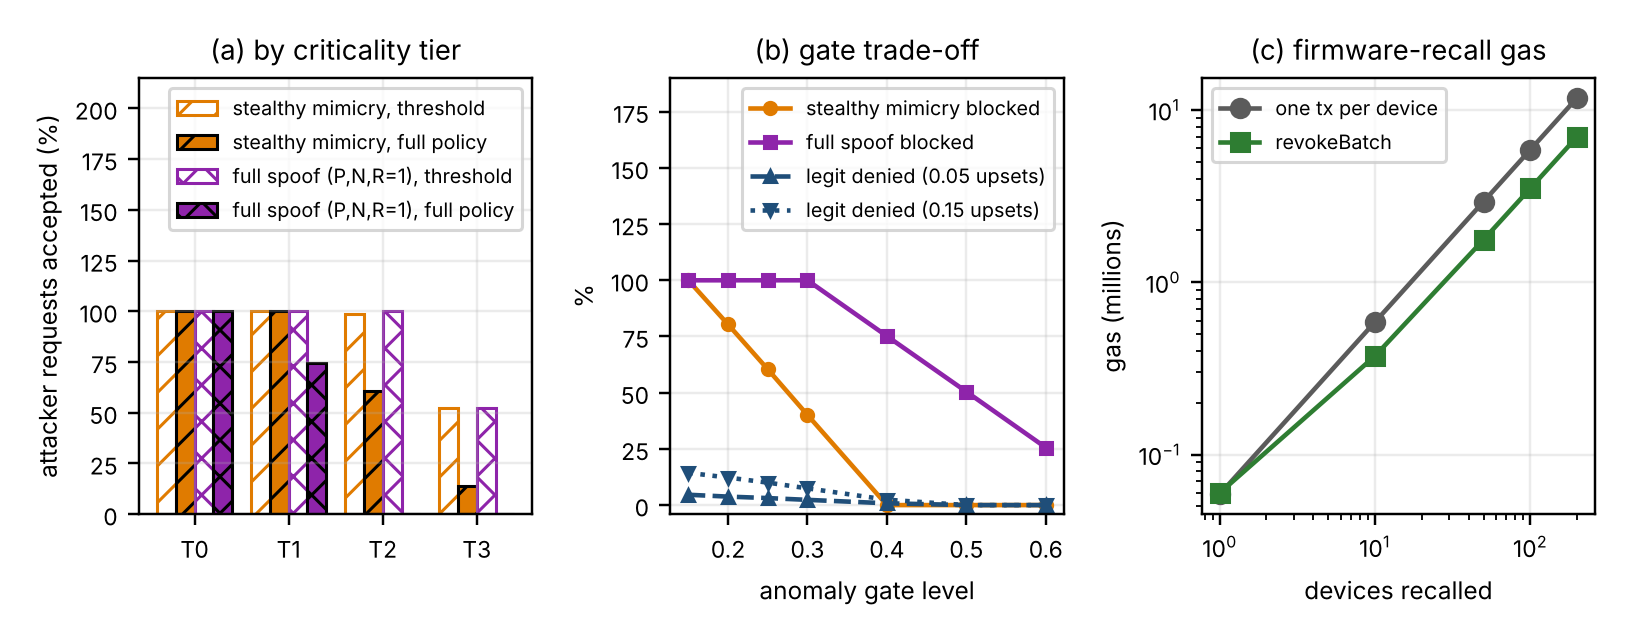
\includegraphics[width=0.72\textwidth]{../figures/fig8_iiot_results.png}
\caption{Industrial extensions: (a) attacker requests accepted per criticality tier under threshold-only and full policy; (b) anomaly-gate trade-off for 5\% and 15\% legitimate process-upset rates; (c) gas to recall devices with one transaction per device versus \texttt{revokeBatch}. Text description: in (a) the full policy accepts fewer attacker requests than the threshold-only policy for at least one attack type at each of T1--T3, and none of the full-spoof requests at T2--T3; in (b) the share of attacks blocked rises with the gate level while the share of legitimate requests denied stays below about 15\%; in (c) recall by \texttt{revokeBatch} uses less gas than one transaction per device for every fleet larger than one device. Bars and lines are distinguished by hatching and markers as well as colour.}
\label{fig:iiotres}
\end{figure*}

\paragraph{WUSTL-IIOT-2018 (SCADA).}\label{sec:wustl_eval} To check that the gate behaviour is not specific to one collection, we repeat the experiment on WUSTL-IIOT-2018 \cite{teixeira2018scada,teixeira2018wustl}. The file has 7{,}037{,}983 rows but only 62{,}959 distinct ones (99.1\% duplicates) and a binary label only, so we de-duplicate before splitting and cannot repeat the held-out-type test. The supervised classifier is almost perfect (AUC 0.99998) because attack flows here are short; an Isolation Forest on normal flows reaches $0.909\pm0.006$, a more realistic stand-in for an unseen attack. With the supervised score the full policy accepts at most 0.3\% of attack requests at T1--T3 and denies at most 0.2\% of legitimate ones. With the unsupervised score it cuts attack acceptance at T2 and T3 from 100\% and 94.1\% to 8.2\% and 4.3\%, but legitimate allowance drops to 87.5\% and 82.2\%, and an adaptive attacker sending its best 10\% (1\%) of flows is accepted 86.9\% (100\%) of the time at T2 and 43.0\% (100\%) at T3, against 2.1\% (16.0\%) and 0.7\% (6.3\%) with the supervised score. With a weak detector the policy trades a large share of legitimate availability for protection at the critical tiers.

\subsection{A Third Dataset With Attack Types: WUSTL-IIoT-2021}\label{sec:wustl21_eval}
WUSTL-IIoT-2021 contains Argus flow records from an industrial Modbus testbed with four labelled attack types \cite{zolanvari2019vulnerability,zolanvari2021wustl}, so it supports the held-out-type test the SCADA file could not. It has 1{,}194{,}464 rows (1{,}107{,}448 normal; DoS 78{,}305, reconnaissance 8{,}240, command injection 259, backdoor 212), captured on one day from two to four attacker hosts. We drop timestamps, IP addresses, the source port, \texttt{IdleTime} (an epoch timestamp that separates types by capture time) and the IP-identification fields, keep 39 features, and remove 41{,}645 exact duplicates. The protocol follows Section~\ref{sec:real_eval}.

The supervised classifier is almost perfect on seen types (AUC 0.99999); the Isolation Forest reaches $0.987\pm0.001$ because normal Modbus polling is very regular. With a type held out, the classifier flags only 0.7\% of DoS test flows at 0.5 (AUC against normal 0.71) and 8.1\% and 13.0\% of command injection and reconnaissance, although their AUC exceeds 0.999. The ranking is right, but the scores sit far below any useful gate. Backdoor is found at 66.7\%. With seen types the full policy admits 3.6--4.2\% of attack requests at T1--T3 and denies no legitimate request. With types withheld, acceptance rises to 75.4--77.8\% on average and 97.9--99.2\% for DoS, so on unseen types the supervised score adds almost nothing, and an adaptive attacker is always accepted. The unsupervised score behaves differently: the full policy admitted no attack request of any type at T1--T3, even for the best 1\% of an adaptive attacker's flows, at the price of denying 1.5\%, 12.1\% and 22.3\% of legitimate requests at T1, T2 and T3. A supervised detector does not protect against unseen attack types, and one trained on normal traffic can, but only when normal traffic is as regular as in this laboratory testbed, whose machine-generated traffic and volumetric attacks make anomaly detection easier than in a plant. The rarest attack types have very few flows (74 and 63 test flows), and posture, network context and device pairing remain synthetic.

\begin{table}[t]
\centering
\caption{WUSTL-IIoT-2021: legitimate requests allowed and attack requests accepted (\%) under the full policy, as means over four attack types; ``Thr.-only'' is the threshold-only policy on the held-out supervised scores}
\label{tab:wustl21}
\scriptsize
\setlength{\tabcolsep}{2.5pt}
\begin{tabular}{@{}lrrrrrr@{}}
\toprule
 & \multicolumn{3}{c}{Supervised $A$} & \multicolumn{2}{c}{Isolation Forest $A$} & \\
\cmidrule(lr){2-4}\cmidrule(lr){5-6}
Tier & Legit & Seen & Held-out & Legit & Attack & Thr.-only$^{a}$ \\
\midrule
T0 & 100.0 & 100.0 & 100.0 & 99.4 & 100.0 & 100.0 \\
T1 & 100.0 & 3.6 & 77.8 & 98.5 & 0.0 & 100.0 \\
T2 & 100.0 & 3.8 & 75.6 & 87.9 & 0.0 & 78.0 \\
T3 & 100.0 & 4.2 & 75.4 & 77.7 & 0.0 & 77.8 \\
\bottomrule
\end{tabular}
\end{table}

\subsection{Baselines: Revocation Exposure, Class Models and Weights}\label{sec:baselines}
On a shared logical clock we compare the per-request design with a session token (HMAC bearer token, TTL 60 or 300\,s) and PKI with a CRL refreshed every 60 or 300\,s, for 60 devices at 1 request/s with revocation times drawn from $U(100,500)$\,s. Table~\ref{tab:base} shows that the audited design accepts no request after revocation, as Proposition~\ref{prop:revoke} predicts, whereas the baselines accept on average 33 and 147 requests for the 60\,s and 300\,s windows (worst cases 59--299). Token validation is cheaper per request, which we do not hide. The fast path trades the zero for a bounded exposure of at most $\rho\Delta$ requests (Proposition~\ref{prop:stale}): with $\Delta=5$\,s and one request per second, 5 requests.

\begin{table}[t]
\centering
\caption{Revocation exposure (requests accepted after revocation; 60 devices, 1 req/s) and mean decision latency}
\label{tab:base}
\scriptsize
\begin{tabular}{@{}lrrr@{}}
\toprule
\textbf{Scheme} & \textbf{Mean exp.} & \textbf{Max exp.} & \textbf{Lat. (ms)} \\
\midrule
Session token (TTL 60 s) & 32.5 & 59 & 0.005 \\
Session token (TTL 300 s) & 146.5 & 299 & 0.006 \\
PKI$+$CRL (refresh 60 s) & 33.5 & 60 & 0.074 \\
PKI$+$CRL (refresh 300 s) & 146.5 & 299 & 0.094 \\
\textbf{Proposed (per-request)} & 0.0 & 0 & 0.070 \\
\bottomrule
\end{tabular}
\end{table}

Three further baselines answer the objection that tokens and CRLs are weak comparators (30 runs, same revocation times). Short-lived certificates and OCSP stapling bound exposure by the validity window because a revoked device cannot renew; in our model they have identical exposure (29.0 requests for 60\,s, 140.8 for 300\,s). A centralised online policy decision point that checks a revocation database on every request matches the audited path with zero exposure, so exposure alone does not favour the blockchain design against it. The differences lie elsewhere. The central PDP is a single operator that alone can revoke, reinstate or silently alter its log, and its log has no external anchor. If it is unreachable for 60\,s it must either deny every request (86.7\% of legitimate requests served) or accept requests from devices revoked meanwhile (21.0 on average, up to 60). Our fast path faces the same outage trade-off for revocations that happen while the replica is blind (Section~\ref{sec:outage_eval}), so the claim we can support concerns governance and auditability, not availability. The simulation models validity windows only.

\paragraph{Architecture-class baselines.}\label{sec:prior_eval} To compare against the \emph{design choices} of earlier blockchain schemes we added two class models, built from how each family is described in the literature and run in the same simulator; they are not re-implementations of any named system. The first is a ledger registry checked at login, after which a session is trusted (the authenticate-once pattern \cite{wang2026medicaliot,james2024authz}): with 60\,s and 300\,s sessions a revoked device is still accepted for a mean of 29.0 and 129.2 requests (maxima 60 and 300). Putting the registry on a ledger therefore does not close the window unless every request is checked. The second is an on-chain policy with one static threshold of 0.55 for every resource. Table~\ref{tab:prior} shows that at the two critical tiers it accepts every partial-mimicry, stealthy and fully spoofed request, since a fully spoofing attacker scores at least 0.70 (Section~\ref{sec:security}), whereas the full policy accepts 0\%, 60.9\% (T2) and 13.6\% (T3) of the three attacks at a cost of 2.2\% and 5.2\% of legitimate requests.

\begin{table}[t]
\centering
\caption{Static single-threshold on-chain policy (class model) versus the full policy at the two critical tiers (synthetic fleet, 4{,}000 requests per population)}
\label{tab:prior}
\scriptsize
\setlength{\tabcolsep}{2.5pt}
\begin{tabular}{@{}llrrrr@{}}
\toprule
& & Legit. & \multicolumn{3}{c}{Attack accepted (\%)} \\
\cmidrule(lr){4-6}
\textbf{Policy} & \textbf{Tier} & denied (\%) & Partial & Stealthy & Full spoof \\
\midrule
Static threshold 0.55 & T2 & 0.0 & 100.0 & 100.0 & 100.0 \\
Full policy (this paper) & T2 & 2.2 & 0.0 & 60.9 & 0.0 \\
Static threshold 0.55 & T3 & 0.0 & 100.0 & 100.0 & 100.0 \\
Full policy (this paper) & T3 & 5.2 & 0.0 & 13.6 & 0.0 \\
\bottomrule
\end{tabular}

\end{table}

\paragraph{Weight sensitivity.} The synthetic weights $(0.30,0.30,0.20,0.20)$ were chosen by hand, so we moved each by $\pm0.10$ (rescaling the others) and drew 200 random perturbations. At T2 legitimate denial stayed between 2.2\% and 2.3\% and stealthy acceptance between 60.5\% and 60.9\%. At T3 legitimate denial ranged from 3.4\% to 11.8\% (median 5.7\%) and stealthy acceptance from 11.8\% to 14.8\%. Partial-mimicry and full-spoof acceptance stayed at 0\% in every variant. The gate therefore holds for any reasonable weighting, while the false-denial cost at the highest tier depends on the weights and should be tuned per plant.

\subsection{Firmware Recall Capacity}\label{sec:recall_eval}
Table~\ref{tab:recall} reports gas for revoking $k$ devices with one transaction each and with \texttt{revokeBatch}; \texttt{suspendBatch} is shown for quarantine. For one device the batch call is 1.7\% dearer, but from ten devices on it saves 36.5--40.5\%, approaching about 35k gas per device against 58.9k. In 30M-gas blocks, recalling $10^4$ devices needs about 20 blocks with individual transactions and 12 with batches, and $5\times10^4$ devices need 99 and 59 (other traffic is not modelled). Devices revoked in later blocks stay exposed until their block, so the highest-criticality devices should go first. A recall approved by quorum adds the vote overhead and executes through \texttt{executeBatch}: 100 devices cost 3.81M gas and 200 devices 7.30M gas in total, about 36.5k gas per device (a fleet of $10^4$ is still about 12 blocks), and a quorum reinstatement with $N=5$ costs 291k gas.

\begin{table}[t]
\centering
\caption{Gas for recalling devices: one transaction per device versus \texttt{revokeBatch}, and \texttt{suspendBatch}}
\label{tab:recall}
\scriptsize
\begin{tabular}{@{}rrrrr@{}}
\toprule
Devices & One tx each & \texttt{revokeBatch} & Saving & \texttt{suspendBatch} \\
\midrule
1 & 58{,}836 & 59{,}859 & -1.7\% & 31{,}626 \\
10 & 588{,}336 & 373{,}725 & 36.5\% & 98{,}907 \\
50 & 2{,}941{,}716 & 1{,}768{,}637 & 39.9\% & 397{,}903 \\
100 & 5{,}883{,}408 & 3{,}512{,}289 & 40.3\% & 771{,}717 \\
200 & 11{,}766{,}864 & 6{,}999{,}533 & 40.5\% & 1{,}519{,}165 \\
\bottomrule
\end{tabular}
\end{table}

\subsection{Attack Detection}\label{sec:attacks}
Replay, forged-signature, use-after-revocation and unregistered-DID probes were each run in 500 trials and denied every time (one-sided 95\% upper bound on failure 0.6\%). This validates the state-machine logic against these attacks; it is not evidence of unconditional security.

\subsection{Decentralized Revocation Governance}\label{sec:governance_eval}
Table~\ref{tab:governance} evaluates \texttt{RevocationGovernance} for $N\in\{5,7,9,11,15,21\}$ with 200 trials per size. Mean quorum latency grows roughly linearly, from 0.56\,ms ($N=5$) to 1.91\,ms ($N=21$) for a cooperative group and from 0.93 to 3.67\,ms under maximal tolerated dissent ($N-q$ DENY voters). In all 1{,}200 trials the dissenting minority never prevented approval, and in 1{,}200 forced-revocation attempts with only $q-1$ approvals no revocation executed, consistent with Proposition~\ref{prop:gov}. On the EVM a proposal costs 76k gas, each vote 78k and the final vote 103k, so a quorum revocation costs 317k ($N=5$) to 805k gas ($N=21$): governance cost grows with $q$, not with the fleet. Kumar et al.\ report 3--4\,s for registration and under 5\,s for revocation on a live PoA chain \cite{kumar2026privacy}; our figures measure compute only and are not comparable like for like. In a deployment each vote is a transaction, so revocation takes about $q$ block confirmations when votes are sequential, or one to two blocks when they are parallel.

\begin{table}[t]
\centering
\caption{Governance: mean testbed latency (ms) cooperative and under maximal dissent; \% trials where maximal dissent still reached quorum (Appr.); \% where a $q-1$ coalition executed a revocation (Forced); EVM gas for one quorum revocation}
\label{tab:governance}
\scriptsize
\begin{tabular}{@{}rrrrrrr@{}}
\toprule
$N$ & $q$ & Coop. & Dissent & Appr.\% & Forced\% & Total gas \\
\midrule
5 & 3 & 0.562 & 0.926 & 100 & 0 & 317{,}162 \\
7 & 4 & 0.667 & 1.166 & 100 & 0 & 378{,}152 \\
9 & 5 & 0.803 & 1.440 & 100 & 0 & 439{,}142 \\
11 & 6 & 0.946 & 1.729 & 100 & 0 & 500{,}120 \\
15 & 8 & 1.299 & 2.438 & 100 & 0 & 622{,}112 \\
21 & 11 & 1.909 & 3.665 & 100 & 0 & 804{,}950 \\
\bottomrule
\end{tabular}
\end{table}

\subsection{End-to-End Evaluation on a Four-Validator QBFT Network}\label{sec:besu_eval}
To move beyond in-process execution we deployed the three contracts on a private Hyperledger Besu 25.7.0 network of four QBFT validators (2\,s block period, 4\,s round-change timeout). We drove it through JSON-RPC with signed transactions. We ran it first with all validators and the load generator on one two-vCPU container, then \label{sec:gcp_eval}on Google Cloud with one validator per e2-standard-2 virtual machine in europe-west3, us-east4, asia-southeast1 and southamerica-east1. We injected no artificial delay and did not record round-trip times, so the delay is whatever the provider's network gave on the day of the run (2026-10-12). Table~\ref{tab:gcp} sets the two runs side by side; both are single runs of the same script.

\emph{Finality and replica lag.} Every state-changing call needs about one block period from submission to receipt (1.98--2.00\,s on average, p95 about 2.2\,s) in both deployments; QBFT finalizes in the block that includes the transaction. Inter-region distance did not push consensus beyond one block period. A revocation became visible on a second validator after 1.87\,s on one host and 1.76\,s across regions, and 30 of 30 audited decisions issued afterwards returned DENY. On one host the replica was up to date before the receipt poll returned ($-117\pm75$\,ms); across regions it trailed the receipt by $+212\pm145$\,ms (p95 362\,ms, maximum 495\,ms). For this network, the exposure bound $\rho\Delta$ of Proposition~\ref{prop:stale} is therefore dominated by the block period plus 0.2--0.5\,s; a plant link over a public network or satellite path would give a larger $\Delta$ and has to be measured where it is deployed.

\emph{Throughput.} Pre-signed audited decisions from ten accounts were all mined at 100, 300 and 600 offered. Sustained throughput was 11--18 tx/s on one host (mean latency 31.6\,s at 600 offered) and 30.8, 34.4 and 50.1 tx/s across regions (8.6\,s). The regional figure is a lower bound, since throughput still rose with load, and both are well below the gas-based ceiling of 213 decisions per second; we did not determine what limits them. We recorded no network round-trip times and did not determine what limits throughput, so the figures describe this setup, not the design's capacity. The conclusion for the design is unchanged: routine requests must not wait for consensus.

\begin{table}[t]
\centering
\caption{The same benchmark on one host and with one validator in each of four Google Cloud regions (mean $\pm$ sd; single runs)}
\label{tab:gcp}
\scriptsize
\setlength{\tabcolsep}{3pt}
\begin{tabular}{@{}lrr@{}}
\toprule
Measurement & One host & Four regions \\
\midrule
Block interval (s) & 2 $\pm$ 0 & 2 $\pm$ 0 \\
\texttt{register}, submit$\to$receipt (ms) & 1977 $\pm$ 139 & 1980 $\pm$ 162 \\
\texttt{evaluateAccess}, submit$\to$receipt (ms) & 1997 $\pm$ 125 & 1997 $\pm$ 134 \\
\texttt{anchorDecisions}, submit$\to$receipt (ms) & 1993 $\pm$ 127 & 1993 $\pm$ 130 \\
Revocation, submit$\to$receipt (ms) & 1985 $\pm$ 121 & 1552 $\pm$ 169 \\
Revocation, submit$\to$visible on replica (ms) & 1868 $\pm$ 85 & 1764 $\pm$ 211 \\
Replica minus receipt (ms) & -117 $\pm$ 75 & 212 $\pm$ 145 \\
Quorum revocation $N{=}5,q{=}3$, sequential (s) & 8.07 $\pm$ 0.24 & 8.17 $\pm$ 0.14 \\
Quorum revocation $N{=}5,q{=}3$, parallel (s) & 4.03 $\pm$ 0.12 & 4.33 $\pm$ 0.13 \\
\texttt{revokeBatch}, 50 devices, receipt (s) & 2.95 & 2.41 \\
\texttt{revokeBatch}, 200 devices, receipt (s) & 6.13 & 2.99 \\
Throughput, 100 offered (tx/s) & 17.8 & 30.8 \\
Throughput, 300 offered (tx/s) & 16.0 & 34.4 \\
Throughput, 600 offered (tx/s) & 11.3 & 50.1 \\
Mean latency at 600 offered (s) & 31.6 & 8.6 \\
\bottomrule
\end{tabular}
\end{table}

\emph{Governance and recall.} A three-of-five revocation took 8.07\,s (one host) and 8.17\,s (regions) with sequential votes, and 4.03\,s and 4.33\,s with parallel votes, about four and two blocks. Revoking 50 and 200 devices in one transaction (1.77M and 7.00M gas) was confirmed after 2.95 and 6.13\,s on one host and 2.41 and 2.99\,s across regions, whereas registering 200 devices one by one took 399\,s. The number of blocks, not the number of transactions, determines recall and governance latency.

\emph{Fault tolerance.} With four validators QBFT tolerates one fault. With one validator stopped, registration averaged 2.83\,s on one host and $3.43\pm2.17$\,s across regions against 1.97\,s at baseline, because rounds in which the stopped validator was the proposer had to time out. With two stopped no block was produced, and a pending transaction was mined 78\,s (one host) and 75\,s (regions) after restart. These runs used one pending transaction and few samples; we did not test partitions, injected delay or validators in one region. During a halt the fast path keeps deciding on its last replicated state, and the outage policy of Section~\ref{sec:outage} governs what is allowed.

\subsection{Ablation, Exposure from the Decision Time, and Calibrated Gates}\label{sec:review_eval}
These three experiments (\texttt{sim/experiments\_review.py}) answer questions that the earlier results left open; all use the same populations, seeds and tiers as above unless stated.

\paragraph{Which component does the work?}\label{sec:ablation2} We compare the full policy with its parts on the synthetic fleet (4{,}000 requests per population, a separate draw from Section~\ref{sec:gate_eval}, so the figures differ slightly). Each alternative is tuned so that it admits the same share of legitimate requests as the full policy, which makes the attack columns comparable. Table~\ref{tab:ablate2} gives the result. The gate carries the effect: at T2 and T3 the threshold alone admits 100\% and 53\% of full spoofing, and adding the gate reduces both to 0\%. Strict mode adds nothing once the gate is present; on its own it only removes the STEP\_UP outcome (at T3 the threshold alone returns ALLOW or STEP\_UP for 85.5\% of full spoofing, against 53.0\% ALLOW). Raising the threshold until legitimate cost matches the gate does not help against full spoofing (58.1\% and 49.0\% still accepted), as Proposition~\ref{prop:bound} predicts. A non-linear score, the minimum of $P$, $1-A$, $N$ and $R$, reaches the same effect without a separate gate (0\% of full spoofing at T2 and T3) and is better than the gate at T1 (38.0\% against 75.3\%). So the evidence supports the principle that the anomaly signal must be able to veto independently of a linear sum; it does not show that a hard gate is the only or best way to do so. Stealthy mimicry, which keeps $A$ low, is not stopped by any variant (18.8--61.1\% still accepted at T2--T3).

\begin{table}[t]
\centering
\caption{Ablation at matched legitimate allowance: attack requests accepted (\%), ALLOW only (4{,}000 requests per population, one seed). Full = gate and strict mode}
\label{tab:ablate2}
\scriptsize
\setlength{\tabcolsep}{3pt}
\begin{tabular}{@{}lrrrrrrrr@{}}
\toprule
& \multicolumn{4}{c}{T2 plc.setpoint.write} & \multicolumn{4}{c}{T3 plc.firmware.update} \\
\textbf{Policy} & Legit. & Partial & Stealthy & Spoof & Legit. & Partial & Stealthy & Spoof \\
\midrule
Threshold only & 99.8 & 53.6 & 98.0 & 100.0 & 95.2 & 7.7 & 53.2 & 53.0 \\
Strict only & 99.8 & 53.6 & 98.0 & 100.0 & 95.2 & 7.7 & 53.2 & 53.0 \\
Gate only & 97.2 & 0.0 & 61.1 & 0.0 & 93.6 & 0.0 & 18.8 & 0.0 \\
Full (gate + strict) & 97.2 & 0.0 & 61.1 & 0.0 & 93.6 & 0.0 & 18.8 & 0.0 \\
Raised threshold & 97.2 & 9.9 & 57.5 & 58.1 & 93.6 & 6.2 & 47.9 & 49.0 \\
Min-of-signals score & 97.2 & 0.0 & 60.7 & 0.0 & 93.6 & 0.0 & 54.6 & 0.0 \\
\bottomrule
\end{tabular}
\end{table}

\paragraph{Exposure counted from the decision time.}\label{sec:exposure_eval} The baselines in Table~\ref{tab:base} count exposure from the moment the revocation is decided, whereas the on-chain figure of zero counts from finalization, which is not a like-for-like comparison. We therefore redraw the revocation delay from the measured Besu distributions (submission to receipt for the audited path, submission to visibility on another validator for the fast path; 30 samples each) and count the requests a device sends at 1 per second after the revocation transaction was \emph{submitted}. Across four regions the audited path accepts 1.5 requests on average (at most 2) and the fast path 1.8 (at most 3); on one host the figures are 2.0 and 1.9 (at most 3 each). The audited and fast paths are therefore indistinguishable in practice, and both are far below the 33 and 147 of the token and CRL baselines (which include no block period at all), though the sample is 30 delays from one run per deployment.

\paragraph{Gates calibrated on legitimate traffic, and a host-grouped split.} The hand-set gates of Table~\ref{tab:tiers} were tuned on synthetic ranges. On TON\_IoT we now split the network flows by source host (35 hosts for training and 16 for testing, five splits), so that no host appears on both sides, and we set one gate at the 99th percentile of half of the legitimate scores, evaluating on the other half. The supervised detector remains strong (AUC 0.999) and the calibrated gate admits 0.4--0.5\% of attack requests with 99.7\% or more of legitimate requests allowed at T1--T3. The Isolation Forest is weaker under this split (AUC 0.874). Its calibrated gate (0.69) lets 91.8, 91.5 and 65.0\% of attack requests through at T1--T3, against 76.9, 40.5 and 34.7\% for the hand-set gates, which cost 2.0, 14.1 and 19.5\% of legitimate requests. On WUSTL-IIoT-2018 with an Isolation Forest trained on normal flows, the hand-set gates admit 100, 9.4 and 4.2\% of attacks while denying 3.6, 13.8 and 18.5\% of legitimate requests. The calibrated gate (0.97) admits 100, 100 and 94.5\% with 1.7, 7.0 and 15.2\% denied. On the original stratified TON\_IoT split with the supervised detector, the calibrated gate (0.27) admits 0.3\% of seen-type attacks and 7.4\% of held-out types on average, but up to 34.6\% for the worst type. A gate set from legitimate data alone therefore cannot be assumed to protect: where attack scores overlap the legitimate tail, the false-denial budget decides how much attack traffic passes, and the gate must be tuned with attack-like data or accepted as weak.

\subsection{Static Analysis and Randomised Invariant Tests}\label{sec:assure}
Slither (102 detectors) reported 11 findings on the three contracts: one medium (a strict equality on \texttt{registeredAt==0}, the intended existence test), four low, one informational finding per signature-recovery routine and four optimisation hints. No reentrancy, access-control or arithmetic finding was reported. Reading the code, we found one genuine gap: with a zero oracle address or a zero registered signer, an invalid signature (for which \texttt{ecrecover} returns the zero address) would pass. We added a zero-oracle check in the constructor and rejected a zero recovered address at registration (+62 gas for \texttt{registerDevice}). Three new tests complement the 13 unit tests, including a randomised state-machine test (300 steps, three seeds, six devices) against an independent model; four further tests cover governor-only revocation, suspend-only single-party action, quorum recall and expired attestations; all 20 pass. The Slither run predates the hardening described in Section~\ref{sec:governance} and has not been repeated. This is bounded random testing, not a proof or audit; the contracts are not formally verified.

\subsection{Degraded Operation During an Outage}\label{sec:outage_eval}
We applied the policy of Section~\ref{sec:outage} to 400 devices at one request per second, a quarter of them T2 clients, with 10\% of devices revoked at random times during an outage starting at $t=200$\,s of 600\,s. A fully fail-closed PEP stops serving everyone, so availability falls to 89.9\% for a 60\,s outage and 50.4\% for 300\,s. The degraded policy keeps T0--T1 running (99.4\% and 97.0\%) but denies every T2 request and accepts requests from devices revoked while it was blind (962 for 60\,s, 4{,}398 for 300\,s). The scenario is deterministic given its parameters, so it illustrates the trade-off rather than measuring it: the operator chooses explicitly between unsafe acceptances and lost availability.

\section{Discussion}\label{sec:disc}

\subsection{What the Design Buys and What It Costs}
Compared with tokens and CRLs, the central gain is the removal of an implicit-trust window: on the audited path a revoked device loses access at the next call, and on the fast path within the replica lag, a bound the operator can set and measure (Propositions~\ref{prop:revoke} and~\ref{prop:stale}; 33--147 accepted requests for the baselines against none or $\rho\Delta$). Quorum governance removes the single-registrar insider (T7) at a gas cost that scales with the voter group rather than the fleet. The tiered policy concentrates verification effort where a wrong decision hurts: at T2--T3 the gate and strict mode cut a spoofing attacker's acceptance from about 100\% to 0\% and from about half to zero, and the cost is a few percent of legitimate requests denied when the process is upset. In contrast to schemes that authenticate once and trust the session \cite{wang2026medicaliot}, nothing here is trusted by default; in contrast to conceptual smart-factory designs \cite{farhan2026ztfsf}, the policy is an executable contract with measured cost.

The costs are equally concrete. The fast path doubles per-request compute (two signature checks), the audited path is bounded by block gas (about 424 decisions per 30M-gas block by gas, and 11--18 per second measured on a single host and 31--50 per second with validators in four regions), recall of very large fleets takes tens of blocks, and the whole design adds a consortium chain, a replica and an oracle to operate. For a plant that has one owner and a good internal PKI, this is probably unjustified; the argument for it is multi-party plants in which revocation authority and audit trails must be shared.

\subsection{Deployment Guidance}
\emph{Tier assignment.} Tiers should follow consequence, not protocol: any action whose misuse could damage equipment or product, or alter safety-relevant logic, belongs on the audited, strict path; high-rate reads belong on the fast path. \emph{Gate calibration.} The anomaly gate should be set from a plant's own distribution of legitimate deviations, including start-up and batch changes (Section~\ref{sec:gate_eval}). \emph{Replica lag.} $\Delta$ should be measured, monitored and alarmed, since Proposition~\ref{prop:stale} is only as good as A5. \emph{Recall rehearsal.} Batch revocation should be rehearsed with quarantine (\texttt{suspendBatch}) first, because REVOKED is terminal and a mistaken revocation requires re-enrolment with a new key. \emph{Privacy and retention.} The ledger should hold identifiers, public keys, status, hashes and trust scores but no personal data; entries are immutable, so anything subject to erasure rules belongs off-chain and is referenced by hash. Status changes and request timing still reveal a plant's inventory and recall activity to every consortium member, so the chain should be permissioned, with read access limited to members. \emph{Keys and clocks.} Device keys belong in a secure element or TPM (A3); any attestation-freshness check needs loosely synchronised clocks in the zone (NTP or PTP) with a stated tolerance. \emph{Gas economics.} On a private PoA network gas can be zero-priced, so the figures above indicate capacity and relative cost rather than money; gasless relaying can hide fees from constrained devices \cite{madhwal2025gasless}.

\subsection{Threats to Validity and Limitations}
\emph{Internal validity.} In the main experiments devices, signals and attacks are synthetic and chosen by us, and the legitimate and attacking anomaly ranges overlap by construction. In the real-data studies only the anomaly signal is real: posture, network context and reliability are synthetic, the assignment of a flow score to a device is arbitrary, and the held-out-type test approximates but is not a real zero-day setting. The datasets have known weaknesses (duplicates, normal and attack records collected on different days, attacks from a few hosts), so the supervised AUC of 0.9999 is optimistic. None of this is a plant measurement. \emph{External validity.} The simulations ran on one two-vCPU container; no measurement was made on a microcontroller or on industrial protocols. The multi-node results come from one single-host run and one four-region run on one provider, on one day, without injected delay or partitions, and the fault tests used a single pending transaction and small samples. The replica lag of about 0.2\,s, the throughput lower bound of 50 tx/s and the failure behaviour have to be measured again on the intended deployment. The legacy-device proxy is a design with a modelled class, not an implemented gateway. \emph{Construct and conclusion validity.} Simulated exposure is counted on a logical clock and ignores propagation and finality time; the Besu runs supply the finality component but not the delay of an industrial network. Intervals come from 10--30 runs; the 500-trial attack tests have a 0.6\% rule-of-three bound.

\emph{Comparison.} No earlier blockchain-IoT or Zero Trust scheme was re-implemented, so the comparison in Table~\ref{tab:relatedwork} is qualitative, and the quantitative baselines (token, CRL, OCSP, central decision point, authenticate-once session, static-threshold policy) are our own class models. Signing and verification were not measured on a constrained device.

\emph{Trust assumptions.} The PEP is trusted for request-signature checking in Track A, and a single oracle and registrar remain single points of compromise (A4); a threshold-signed oracle \cite{hassan2023oracle} and a quorum registrar set would remove them. Multi-PEP zones require binding the PEP identity into requests (Proposition~\ref{prop:replay}). Trust scores appear in transaction data and are visible to consortium members; differential-privacy protection of exposed scores \cite{ren2026ditdp} is not implemented.

\emph{Detection.} A detector-dependent gate inherits the detector's blind spots on unseen attacks and is exposed to an adaptive attacker who can steer its own score. Adversarially robust detection, rate limiting of low-score probing and joint use of several detectors are natural defences that we did not evaluate; adversarial-AI mimicry is richer than our populations \cite{usama2026multilayer}, and the signal producers (attestation, process-aware anomaly detection, possibly cross-site learning \cite{tom2025flcti}) are inputs we assume. Learning the hand-tuned policy parameters from plant data \cite{salim2026ztblociot} is open, as is a field study joining per-device telemetry to the traffic of the same device.

\emph{Contracts.} The contracts are research code. They pass 20 tests, and a Slither run on the earlier version found no serious issue after one hardening fix (it was not repeated after the governance change), but they have not been audited or formally verified; the literature on smart-contract quality assurance \cite{wei2024quality} should be followed before any production use.

\section{Conclusion}\label{sec:concl}
A plant needs three things from an identity system: revocation authority shared among its organizations, verification proportional to the consequence of a request, and an enforcement path that does not wait for consensus. We built one around three smart contracts for identity, tiered policy and quorum-governed revocation. Routine requests are decided locally against replicated state, and their decision logs are anchored as Merkle roots; costly requests are decided on-chain with an anomaly gate and a strict mode; batch revocation handles firmware recalls. We proved immediate revocation on the audited path, a $\rho\Delta$ exposure bound on the fast path (conditional on the replica-lag assumption), replay resistance, attestation unforgeability with an expiry time, key-reuse prevention, and governance safety (liveness needs $q$ participating voters). We also stated when a spoofing attacker passes the gate. After the review we also made revocation, reinstatement and recall quorum-only, so a single party can only suspend a device.

The measurements support the design with limits. In simulation, the audited path denied every request after finality, and counted from the submission of the revocation both paths accepted about two requests at one request per second, where token and CRL baselines accepted 33--147 on average. At the two most critical tiers, the gate brought full-spoof acceptance to 0\% and stealthy-mimicry acceptance to 18.8--61.1\% at a cost of 2.2--5.2\% of legitimate requests denied; an ablation shows that the gate (or an equivalent non-linear veto) is what does this, and that strict mode adds nothing once a gate is present. Batch revocation saved about 40\% of gas, and a quorum revocation cost 313k--800k gas for 5--21 voters. With the behavioural signal taken from real traffic, the gate was only as good as the detector behind it. A supervised detector accepted 75--78\% of attack requests of withheld types at the upper tiers of one dataset. A detector trained on normal traffic blocked them but denied 12--22\% of legitimate requests at the two critical tiers, and gates calibrated on legitimate traffic alone let 65--100\% of attacks through for such a detector. An adaptive attacker that sent only its best-scoring flows was accepted 29--77\% of the time on TON\_IoT. An attacker that keeps its behaviour within normal variation is accepted at every tier. A centralised online decision point also matches the zero exposure of the audited path, so the case for this design rests on shared revocation authority and an externally anchored audit trail, not on exposure alone.

On a four-validator Besu QBFT network, audited calls were final in about one 2\,s block. A revocation was visible on a second validator after about 1.9\,s on one host and 1.8\,s across four Google Cloud regions, where it reached a remote validator about 0.2\,s after the submitting node's receipt, and it denied all 30 later audited requests. A three-of-five quorum revocation took 4--8\,s. Sustained throughput was 11--18 decisions per second on one two-vCPU host and at least 31--50 across regions. With two of four validators stopped the chain halted safely, as intended. These are single runs on the contract version before the governance hardening. No round-trip times were recorded, the throughput limit was not determined, and the virtual machines have been deleted, so the runs cannot be repeated. The timing figures of the in-process testbed are compute-bound, and the posture and network signals remain synthetic.

The architecture relies on an external detector and a trust oracle, which it neither provides nor secures. Whether the approach holds up in a real plant has to be settled on a plant network, with real protocols, devices and telemetry. We regard that as the next step, together with threshold-signed oracles, key rotation and voter-set changes (not implemented), and privacy protection for exposed scores. Code, result files and generation scripts are at \href{https://github.com/irfanrazanaqvi/BCZT_IDM_IoT_experments_code}{github.com/irfanrazanaqvi/BCZT\_IDM\_IoT\_experments\_code}; the TON\_IoT and WUSTL data must be obtained from their owners.


\newcommand{\confirm}{\textcolor{red}{[AUTHORS TO CONFIRM]}}
\section*{CRediT authorship contribution statement}
\textbf{Syed Irfan Raza Naqvi:} Conceptualization, Methodology, Software, Validation, Formal analysis, Investigation, Data curation, Writing -- original draft, Visualization \confirm.
\textbf{Muhammad Umar Aftab:} Supervision, Conceptualization, Writing -- review \& editing \confirm.
\textbf{Rana Asif Rehman:} \textcolor{red}{[roles to be completed by the author]}.
\textbf{Ahmad Mohsin:} \textcolor{red}{[roles to be completed by the author]}.
\textbf{Sayed Qaiser Ali Shah:} \textcolor{red}{[roles to be completed by the author]}.

\section*{Declaration of competing interest}
The authors declare that they have no known competing financial interests or personal relationships that could have appeared to influence the work reported in this paper. \confirm

\section*{Funding}
This research did not receive any specific grant from funding agencies in the public, commercial, or not-for-profit sectors. \confirm

\section*{Data availability}
The contracts, simulation and experiment scripts, and all result files are openly available at \href{https://github.com/irfanrazanaqvi/BCZT_IDM_IoT_experments_code}{github.com/irfanrazanaqvi/BCZT\_IDM\_IoT\_experments\_code}. The TON\_IoT and WUSTL-IIoT datasets are third-party resources and must be obtained from their owners under their licences.

\section*{Declaration of generative AI and AI-assisted technologies in the writing process}
During the preparation of this work the authors used Claude (Anthropic) to assist with drafting and editing text, generating and debugging experiment and figure code, and organising the reference list. After using this tool, the authors reviewed and edited the content as needed and take full responsibility for the content of the publication. \confirm


\begingroup\small\setstretch{1.0}
\begin{thebibliography}{99}\small
\setlength{\itemsep}{0pt}
\setlength{\parskip}{0pt}
\small
\setlength{\itemsep}{0pt}
\setlength{\parskip}{0pt}
\bibitem{stouffer2023sp80082}
K. Stouffer \emph{et al.}, ``Guide to Operational Technology (OT) Security,'' NIST Special Publication 800-82 Rev.~3, National Institute of Standards and Technology, Sep. 2023. \href{https://doi.org/10.6028/NIST.SP.800-82r3}{doi:\nolinkurl{10.6028/NIST.SP.800-82r3}}

\bibitem{nist800207}
S. Rose, O. Borchert, S. Mitchell, and S. Connelly, ``Zero Trust Architecture,'' NIST Special Publication 800-207, National Institute of Standards and Technology, 2020. \href{https://doi.org/10.6028/NIST.SP.800-207}{doi:\nolinkurl{10.6028/NIST.SP.800-207}}

\bibitem{fernandez2024critical}
E. B. Fernandez and A. Brazhuk, ``A critical analysis of zero trust architecture (ZTA),'' \emph{Computer Standards \& Interfaces}, vol. 89, Art. no. 103832, 2024. \href{https://doi.org/10.1016/j.csi.2024.103832}{doi:\nolinkurl{10.1016/j.csi.2024.103832}}

\bibitem{phiayura2023comprehensive}
P. Phiayura and S. Teerakanok, ``A comprehensive framework for migrating to zero trust architecture,'' \emph{IEEE Access}, vol. 11, pp. 19487--19511, 2023. \href{https://doi.org/10.1109/ACCESS.2023.3248622}{doi:\nolinkurl{10.1109/ACCESS.2023.3248622}}

\bibitem{song2025ztot}
M. W. Song, T. Nguyen, and C. Irvine, ``A zero trust architecture for critical operational technology systems,'' in \emph{Proc. 58th Hawaii Int. Conf. Syst. Sci. (HICSS)}, 2025. \href{https://doi.org/10.24251/HICSS.2025.849}{doi:\nolinkurl{10.24251/HICSS.2025.849}}

\bibitem{zanasi2024flexible}
C. Zanasi, S. Russo, and M. Colajanni, ``Flexible zero trust architecture for the cybersecurity of industrial IoT infrastructures,'' \emph{Ad Hoc Networks}, vol. 156, Art. no. 103414, 2024. \href{https://doi.org/10.1016/j.adhoc.2024.103414}{doi:\nolinkurl{10.1016/j.adhoc.2024.103414}}

\bibitem{w3cdid2022}
M. Sporny \emph{et al.}, ``Decentralized Identifiers (DIDs) v1.0,'' W3C Recommendation, Jul. 2022. \href{https://www.w3.org/TR/did-core/}{w3.org/TR/did-core}

\bibitem{hosseini2023blockchain}
S. M. Hosseini, J. Ferreira, and P. C. Bartolomeu, ``Blockchain-based decentralized identification in IoT: an overview of existing frameworks and their limitations,'' \emph{Electronics}, vol. 12, no. 6, p. 1283, 2023. \href{https://doi.org/10.3390/electronics12061283}{doi:\nolinkurl{10.3390/electronics12061283}}

\bibitem{aguru2025ssi}
A. D. Aguru and S. B. Erukala, ``A blockchain-based self-sovereign identity management framework for Internet of Things,'' in \emph{Recent Trends in Intelligent Systems and Next Generation Wireless Communication (IIWCS 2024)}, Lecture Notes in Networks and Systems, vol. 1329. Singapore: Springer, 2025, pp. 299--309. \href{https://doi.org/10.1007/978-981-96-4741-5_26}{doi:\nolinkurl{10.1007/978-981-96-4741-5_26}}

\bibitem{folino2025puf}
G. Folino, A. Forestiero, and G. Papuzzo, ``Self-sovereign identification of IoT devices by using physically unclonable functions and blockchain,'' in \emph{Numerical Computations: Theory and Algorithms (NUMTA 2023)}, Lecture Notes in Computer Science, vol. 14478. Cham: Springer, 2025. \href{https://doi.org/10.1007/978-3-031-81247-7_26}{doi:\nolinkurl{10.1007/978-3-031-81247-7_26}}

\bibitem{zhai2025chebyshev}
Z. Zhai \emph{et al.}, ``A lightweight authentication method for Industrial Internet of Things based on blockchain and Chebyshev chaotic maps,'' \emph{Future Internet}, vol. 17, no. 8, Art. no. 338, 2025. \href{https://doi.org/10.3390/fi17080338}{doi:\nolinkurl{10.3390/fi17080338}}

\bibitem{essaid2025iiotbc}
M. Essaid and H. Ju, ``Blockchain solutions for enhancing security and privacy in Industrial IoT,'' \emph{Applied Sciences}, vol. 15, no. 12, Art. no. 6835, 2025. \href{https://doi.org/10.3390/app15126835}{doi:\nolinkurl{10.3390/app15126835}}

\bibitem{liu2024dissecting}
C. Liu, R. Tan, Y. Wu, Y. Feng, Z. Jin, F. Zhang, Y. Liu, and Q. Liu, ``Dissecting zero trust: research landscape and its implementation in IoT,'' \emph{Cybersecurity}, vol. 7, no. 1, Art. no. 20, 2024. \href{https://doi.org/10.1186/s42400-024-00212-0}{doi:\nolinkurl{10.1186/s42400-024-00212-0}}

\bibitem{nie2025zeroTrust}
S. Nie, J. Ren, R. Wu, P. Han, Z. Han, and W. Wan, ``Zero-trust access control mechanism based on blockchain and inner-product encryption in the Internet of Things in a 6G environment,'' \emph{Sensors}, vol. 25, no. 2, p. 550, 2025. \href{https://doi.org/10.3390/s25020550}{doi:\nolinkurl{10.3390/s25020550}}

\bibitem{salim2026ztblociot}
M. M. Salim, M. Kim, S. K. Singh, and J. H. Park, ``Zero-trust blockchain-enabled framework for scalable and secure IoT networks (ZT-BlocIoT),'' \emph{Future Generation Computer Systems}, vol. 175, Art. no. 108093, 2026. \href{https://doi.org/10.1016/j.future.2025.108093}{doi:\nolinkurl{10.1016/j.future.2025.108093}}

\bibitem{mukta2026ztdelegation}
R. Mukta, S. Pal, K. Chowdhury, M. Hitchens, H. Paik, and S. S. Kanhere, ``Zero trust-driven access control delegation using blockchain,'' \emph{Blockchain: Research and Applications}, vol. 7, no. 1, Art. no. 100319, 2026. \href{https://doi.org/10.1016/j.bcra.2025.100319}{doi:\nolinkurl{10.1016/j.bcra.2025.100319}}

\bibitem{jamwal2026survey}
E. Jamwal, P. Srivastava, and P. S. Chakraborty, ``Blockchain-enabled zero-trust framework for secure cloud data sharing: survey,'' in \emph{Proc. 2026 Int. Conf. Intell. Syst. Eng., Secured Syst. Cybersecurity (ICISESSC)}, 2026. \href{https://doi.org/10.1109/ICISESSC68634.2026.11542695}{doi:\nolinkurl{10.1109/ICISESSC68634.2026.11542695}}

\bibitem{farhan2026ztfsf}
M. Farhan \emph{et al.}, ``ZTF-SF: a zero-trust blockchain-enabled IIoT framework for secure smart factories,'' in \emph{Proc. 2026 2nd Int. Conf. Comput. Intell. Approaches Appl. (ICCIAA)}, 2026. \href{https://doi.org/10.1109/ICCIAA68481.2026.11543806}{doi:\nolinkurl{10.1109/ICCIAA68481.2026.11543806}}

\bibitem{potturi2026hybrid}
K. Potturi, B. Gautam, C. S. Pareek, A. Gupta, S. C. Chava, and B. S. Katta, ``A hybrid AI and blockchain-enabled zero-trust security framework for cloud, edge, and IoT systems,'' in \emph{Proc. 2026 Int. Conf. Comput. Theory Wireless Commun. (ICCTWC)}, 2026. \href{https://doi.org/10.1109/ICCTWC68241.2026.11582964}{doi:\nolinkurl{10.1109/ICCTWC68241.2026.11582964}}

\bibitem{wang2026medicaliot}
Z. Wang, Y. Guo, and Y. Guo, ``Blockchain-based zero-trust continuous authentication scheme for medical IoT,'' \emph{Journal of Parallel and Distributed Computing}, vol. 217, Art. no. 105333, 2026. \href{https://doi.org/10.1016/j.jpdc.2026.105333}{doi:\nolinkurl{10.1016/j.jpdc.2026.105333}}

\bibitem{james2024authz}
M. James, T. Newe, D. O'Shea, and G. D. O'Mahony, ``Authentication and authorization in zero trust IoT: A survey,'' in \emph{Proc. Irish Signals and Systems Conf. (ISSC)}, 2024. \href{https://doi.org/10.1109/ISSC61953.2024.10603175}{doi:\nolinkurl{10.1109/ISSC61953.2024.10603175}}

\bibitem{kumar2024industry40}
R. Kumar and R. Sharma, ``A comprehensive approach to industry 4.0 security: blockchain and dynamic access control integration,'' in \emph{Proc. 2024 6th Int. Conf. Computational Intelligence and Communication Technologies (CCICT)}, 2024, pp. 477--484. \href{https://doi.org/10.1109/CCICT62777.2024.00080}{doi:\nolinkurl{10.1109/CCICT62777.2024.00080}}

\bibitem{azad2024verify}
M. A. Azad, S. Abdullah, J. Arshad, H. Lallie, and Y. H. Ahmed, ``Verify and trust: a multidimensional survey of zero-trust security in the age of IoT,'' \emph{Internet of Things}, vol. 27, Art. no. 101227, 2024. \href{https://doi.org/10.1016/j.iot.2024.101227}{doi:\nolinkurl{10.1016/j.iot.2024.101227}}

\bibitem{nahar2024survey}
N. Nahar, K. Andersson, O. Schel\'en, and S. Saguna, ``A survey on zero trust architecture: applications and challenges of 6G networks,'' \emph{IEEE Access}, vol. 12, pp. 94753--94764, 2024. \href{https://doi.org/10.1109/ACCESS.2024.3425350}{doi:\nolinkurl{10.1109/ACCESS.2024.3425350}}

\bibitem{prezta2026}
Z. Wei, O. M. Ameer, Y. Zhang, and N. Borisov, ``PREZTA: Provable remote execution of zero-trust authorization using SNARKs,'' arXiv:2607.11466, 2026. \href{https://doi.org/10.48550/arXiv.2607.11466}{doi:\nolinkurl{10.48550/arXiv.2607.11466}}

\bibitem{ren2025aiot}
J. Ren, J. Zhang, Y. Ren, and J. Xu, ``Blockchain-based self-sovereign identity management mechanism in AIoT environments,'' \emph{Electronics}, vol. 14, no. 19, p. 3954, 2025. \href{https://doi.org/10.3390/electronics14193954}{doi:\nolinkurl{10.3390/electronics14193954}}

\bibitem{ali2025dtaccess}
G. Ali, S. Shah, M. Elaffendi, and N. Ahmad, ``Blockchain-based access management framework for interoperable digital twins in industrial IoT,'' \emph{Frontiers in Blockchain}, vol. 8, Art. no. 1693926, 2025. \href{https://doi.org/10.3389/fbloc.2025.1693926}{doi:\nolinkurl{10.3389/fbloc.2025.1693926}}

\bibitem{philipp2023daxiot}
A. Philipp and A. K\"upper, ``DAXiot: A decentralized authentication and authorization scheme for dynamic IoT networks,'' arXiv:2307.06919, 2023. \href{https://doi.org/10.48550/arXiv.2307.06919}{doi:\nolinkurl{10.48550/arXiv.2307.06919}}

\bibitem{mazzocca2024evoke}
C. Mazzocca, A. Acar, S. Uluagac, and R. Montanari, ``EVOKE: Efficient revocation of verifiable credentials in IoT networks,'' in \emph{Proc. 33rd USENIX Security Symp.}, Philadelphia, PA, USA, Aug. 2024, pp. 1279--1295. \href{https://www.usenix.org/system/files/usenixsecurity24-mazzocca.pdf}{usenix.org (PDF)}

\bibitem{kumar2026privacy}
A. Kumar, B. Sharma, R. K. Kaushal, and I. Ben Dhaou, ``Privacy-preserving identity management system leveraging blockchain technology,'' in \emph{Proc. 15th IEEE Int. Conf. Commun. Syst. Netw. Technol. (CSNT)}, 2026, pp. 625--631. \href{https://doi.org/10.1109/CSNT69054.2026.11502058}{doi:\nolinkurl{10.1109/CSNT69054.2026.11502058}}

\bibitem{rivera2026yangbaxter}
Y. E. Rivera-Julio, E. A. Leal-Narv\'aez, and J. Prieto Tejedor, ``Blockchain-backed revocation and Yang--Baxter consistency screening for zero-trust IoT admission control,'' \emph{Sensors}, vol. 26, no. 18, Art. no. 5960, 2026. \href{https://doi.org/10.3390/s26185960}{doi:\nolinkurl{10.3390/s26185960}}

\bibitem{usama2026multilayer}
M. Usama, A. Aziz, N. Alasbali, N. Alturki, M. Hanif, and M. Ur Rehman, ``Blockchain-enabled identity management for IoT: a multi-layered defense against adversarial AI,'' \emph{Scientific Reports}, vol. 16, Art. no. 4371, 2026. \href{https://doi.org/10.1038/s41598-026-35208-y}{doi:\nolinkurl{10.1038/s41598-026-35208-y}}

\bibitem{tom2025flcti}
A. K. Tom, A. Khraisat, T. Jan, M. Whaiduzzaman, T. D. Nguyen, and A. Alazab, ``Survey of federated learning for cyber threat intelligence in Industrial IoT: Techniques, applications and deployment models,'' \emph{Future Internet}, vol. 17, no. 9, Art. no. 409, 2025. \href{https://doi.org/10.3390/fi17090409}{doi:\nolinkurl{10.3390/fi17090409}}

\bibitem{shujaa2025enhancing}
W. Shujaa, M. Alanzi, and S. Sankaranarayanan, ``Enhancing IoT security through blockchain integration,'' \emph{Frontiers in Computer Science}, vol. 7, Art. no. 1670473, 2025. \href{https://doi.org/10.3389/fcomp.2025.1670473}{doi:\nolinkurl{10.3389/fcomp.2025.1670473}}

\bibitem{hassan2023oracle}
A. Hassan, I. Makhdoom, W. Iqbal, A. Ahmad, and A. Raza, ``From trust to truth: Advancements in mitigating the blockchain oracle problem,'' \emph{J. Netw. Comput. Appl.}, vol. 217, Art. no. 103672, 2023. \href{https://doi.org/10.1016/j.jnca.2023.103672}{doi:\nolinkurl{10.1016/j.jnca.2023.103672}}

\bibitem{wei2024quality}
Z. Wei \emph{et al.}, ``Survey on quality assurance of smart contracts,'' \emph{ACM Comput. Surv.}, vol. 57, no. 2, Art. no. 32, 2024. \href{https://doi.org/10.1145/3695864}{doi:\nolinkurl{10.1145/3695864}}

\bibitem{ta2024gascost}
M. T. Ta and T. Q. Do, ``A study on gas cost of Ethereum smart contracts and performance of blockchain on simulation tool,'' \emph{Peer-to-Peer Networking and Applications}, vol. 17, no. 1, pp. 200--212, 2024. \href{https://doi.org/10.1007/s12083-023-01598-3}{doi:\nolinkurl{10.1007/s12083-023-01598-3}}

\bibitem{hasan2023smartcontract}
M. R. Hasan, A. Alazab, S. B. Joy, M. N. Uddin, M. A. Uddin, A. Khraisat, I. Gondal, W. F. Urmi, and M. A. Talukder, ``Smart contract-based access control framework for Internet of Things devices,'' \emph{Computers}, vol. 12, no. 11, Art. no. 240, 2023. \href{https://doi.org/10.3390/computers12110240}{doi:\nolinkurl{10.3390/computers12110240}}

\bibitem{haque2024scalable}
E. U. Haque, A. Shah, J. Iqbal, S. S. Ullah, R. Alroobaea, and S. Hussain, ``A scalable blockchain based framework for efficient IoT data management using lightweight consensus,'' \emph{Scientific Reports}, vol. 14, Art. no. 7841, 2024. \href{https://doi.org/10.1038/s41598-024-58578-7}{doi:\nolinkurl{10.1038/s41598-024-58578-7}}

\bibitem{peepliwal2024ztab}
A. K. Peepliwal, H. M. Pandey, S. Prakash, A. A. Mahajan, S. S. Chowhan, V. Kumar, and R. Sharma, ``A prototype model of zero trust architecture blockchain with EigenTrust-based practical Byzantine fault tolerance protocol to manage decentralized clinical trials,'' \emph{Digital Communications and Networks}, 2024. \href{https://www.sciencedirect.com/science/article/pii/S2096720924000459}{sciencedirect.com (S2096720924000459)}

\bibitem{madhwal2025gasless}
Y. Madhwal \emph{et al.}, ``Empowering autonomous IoT devices in blockchain through gasless transactions,'' \emph{Blockchain: Research and Applications}, vol. 6, no. 2, Art. no. 100257, 2025. \href{https://doi.org/10.1016/j.bcra.2024.100257}{doi:\nolinkurl{10.1016/j.bcra.2024.100257}}

\bibitem{ren2026ditdp}
L. Ren, H. Li, Y. Liu, D. Liao, M. Zhang, and H. Jin, ``Identity trust management based on differential privacy for internet of vehicles,'' \emph{Scientific Reports}, vol. 16, Art. no. 20921, 2026. \href{https://doi.org/10.1038/s41598-026-50273-z}{doi:\nolinkurl{10.1038/s41598-026-50273-z}}

\bibitem{alsaedi2020ton}
A. Alsaedi, N. Moustafa, Z. Tari, A. Mahmood, and A. Anwar, ``TON\_IoT telemetry dataset: A new generation dataset of IoT and IIoT for data-driven intrusion detection systems,'' \emph{IEEE Access}, vol. 8, pp. 165130--165150, 2020. \href{https://doi.org/10.1109/ACCESS.2020.3022862}{doi:\nolinkurl{10.1109/ACCESS.2020.3022862}}

\bibitem{moustafa2021network}
N. Moustafa, ``A new distributed architecture for evaluating AI-based security systems at the edge: Network TON\_IoT datasets,'' \emph{Sustainable Cities and Society}, vol. 72, Art. no. 102994, 2021. \href{https://doi.org/10.1016/j.scs.2021.102994}{doi:\nolinkurl{10.1016/j.scs.2021.102994}}

\bibitem{booij2022ton}
T. M. Booij, I. Chiscop, E. Meeuwissen, N. Moustafa, and F. T. H. den Hartog, ``ToN\_IoT: The role of heterogeneity and the need for standardization of features and attack types in IoT network intrusion data sets,'' \emph{IEEE Internet Things J.}, vol. 9, no. 1, pp. 485--496, 2022. \href{https://doi.org/10.1109/JIOT.2021.3085194}{doi:\nolinkurl{10.1109/JIOT.2021.3085194}}

\bibitem{teixeira2018scada}
M. A. Teixeira, T. Salman, M. Zolanvari, R. Jain, N. Meskin, and M. Samaka, ``SCADA system testbed for cybersecurity research using machine learning approach,'' \emph{Future Internet}, vol. 10, no. 8, Art. no. 76, 2018. \href{https://doi.org/10.3390/fi10080076}{doi:\nolinkurl{10.3390/fi10080076}}

\bibitem{teixeira2018wustl}
M. A. Teixeira, M. Zolanvari, and R. Jain, ``WUSTL-IIOT-2018 dataset for ICS (SCADA) cybersecurity research,'' IEEE DataPort, 2018. \href{https://doi.org/10.21227/kzgp-7t84}{doi:\nolinkurl{10.21227/kzgp-7t84}}

\bibitem{zolanvari2019vulnerability}
M. Zolanvari, M. A. Teixeira, L. Gupta, K. M. Khan, and R. Jain, ``Machine learning-based network vulnerability analysis of industrial Internet of Things,'' \emph{IEEE Internet Things J.}, vol. 6, no. 4, pp. 6822--6834, 2019. \href{https://doi.org/10.1109/JIOT.2019.2912022}{doi:\nolinkurl{10.1109/JIOT.2019.2912022}}

\bibitem{zolanvari2021wustl}
M. Zolanvari, ``WUSTL-IIOT-2021,'' IEEE DataPort, 2021. \href{https://doi.org/10.21227/yftq-n229}{doi:\nolinkurl{10.21227/yftq-n229}}

\end{thebibliography}
\endgroup
\end{document}

\end{document}
